\documentclass[fleqn, handout, 10pt]{beamer}


\title{\textbf{Stata Training}}
\date[July 2013]{July 31, 2013}
\author[J. Fogel]{Jamie Fogel \\ Federal Reserve Bank of Boston \\ }

\def\tex{S:/trainings/stata/tex}
\def\results{S:/trainings/exporting_stata_tables_figures/results}


\usetheme{AnnArbor}
\usecolortheme{wolverine}

\setbeamertemplate{footline}
{%
  \begin{beamercolorbox}{section in head/foot}
	\hspace{1em} \insertshortauthor \hfill \inserttitle , \insertshortdate \hfill \insertframenumber /  \inserttotalframenumber \hspace{1em}
  \end{beamercolorbox}%
}




\usepackage{hyperref}
\usepackage{import}
\usepackage{caption}
\captionsetup{labelformat=empty,labelsep=none}
\usepackage{amsmath}
\setlength{\mathindent}{0.5 em}
\usepackage{wrapfig}
\usepackage{comment}
\usepackage{listings}
\usepackage{booktabs}

%\usepackage{subfig}


\usebeamercolor{structure}
\usebeamercolor{frametitle}
%\setbeamercolor{block title}{bg=\color{structure.fg}, fg=black}

\lstset{basicstyle= \ttfamily \scriptsize, frame=trbl, backgroundcolor=\color{frametitle.bg},rulecolor=\color{structure.fg}}
\usepackage{xcolor}

\def\lst{\lstinline}

\setlength{\parskip}{10pt}
\newcommand{\com}[1]{{\footnotesize\texttt{#1}}}
\renewcommand{\thefootnote}{\roman{footnote}}

\begin{document}


\section{Introduction}

\begin{frame}[plain]
    \titlepage \let\thefootnote\relax\footnote{This presentation borrows heavily from Ryan Kessler's Stata training, Summer 2012}
\end{frame}

\subsection{Basic Rules for Stata Success}

\begin{frame}{Basic Rules for Stata Success}
    \begin{enumerate}
	\item All of your work should be in a do-file \pause
	\item Use loops and macros to keep your code simple \pause
    \item Add comments to your code to keep it organized and make it easy for others (or yourself a year later) to understand \pause
	\item Use a log file \pause
	\item Set up an organized file structure
    \end{enumerate}
\end{frame}

\begin{frame}{All of your work should be in a do-file}
	\begin{itemize}
	    \item You \textbf{\emph{ALWAYS}} want to have a record of what you are doing; a do-file is that record
	    \item You may be asked to update your results months from now, after new data has been released. With a do-file this is as simple as re-running your code with the updated data.  \pause
	\end{itemize}
    \centering
	    \begin{wrapfigure}{r}{.4\textwidth}
		\begin{center}
		\includegraphics[width=.4\textwidth]{S:/misc_results/dofile_badtime.eps}
		\end{center}
	    \end{wrapfigure}
	\clearpage
\end{frame}

\section{Logic and Logical (Boolean) Operators}

\begin{frame}[fragile]{Boolean}
    \begin{itemize}
        \item In most programming languages, including Stata, a \textbf{Boolean}, or logical, is a data type that takes only two possible values: true or false.
        \item A Boolean expression evaluates to 0 if false or 1 if true.
    \end{itemize}\pause
    \begin{lstlisting}
di 1==1
> 1
di 1==0
> 0
    \end{lstlisting}
\end{frame}

\begin{frame}[fragile]{Boolean expressions}
    In programming ``=='' tests for equality, while ``='' is used for assigning values to variables. \pause
    \begin{lstlisting}
set obs 1
gen x = 1
count if x == 1
> 1
gen y == 1
> == invalid name
> r(198);
	    \end{lstlisting}
\pause
    The operators +==, ~=, !=, >, >=, <,+ and \lst+<=+ are used to test equality or inequality. The operators \lst+& | ~+ and \lst+!+ are used to indicate ``and'', ``or'', and ``not''.
\end{frame}

\begin{frame}[fragile]{Boolean arguments}
    \begin{itemize}
        \item Logical or Boolean arguments, such as the argument to \lst=if= or \lst=while=, may take on any value, not just 0 or 1
        \item 0 is treated as false and any other numeric value as true
    \end{itemize} \pause
    \begin{lstlisting}
local a = 35
if `a'    di `a'
> 35
local a = 0
if `a'    di `a'
>
    \end{lstlisting}
\end{frame}

\begin{frame}{Missing valuse}
    Be careful: \textbf{Missing evaluates to true!!!} Remember, as far as an \lst=if= or \lst=while= statement is concerned, 0 means false and anything else means true. Stata's missing value indicator, ``.'', evaluates to infinity; infinity is not 0 and therefore must mean true. This is simple, but it is something you are very likely to encounter.
\end{frame}

\begin{frame}{A useful resource}
    Much of the language on the preceding slides was taken from the below Stata support page. I recommend you visit it if you have any further questions.
    \url{http://www.stata.com/support/faqs/data-management/true-and-false/}
\end{frame}
\section{Macros}

\subsection{A Quick Review}
\begin{frame}[fragile]{Macros}
    A Stata macro is what most programming languages call a variable; they can be used to store content, numeric or string, which can then be inserted elsewhere in the code by invoking the macro. Macros can be local or global in scope, with the former existing solely within the program or do-file in which they are defined and the latter remaining available until they are dropped (\lst=macro drop macroname=) or Stata is closed.

    Local macros are invoked by placing the macroname between a backtick (`) and a forward tick ('); global macros are invoked by preceding the macroname with the dollar sign (\$). In either case, braces (\{\}) can be used to clarify meaning and to form nested constructions. For example:

    \begin{columns}[t]
    \centering
	\column{.5\textwidth}
	    \begin{lstlisting}
* Local macros
local l1 "p"
local l2 "i"
gen `l1'`l2' = c(pi)
	    \end{lstlisting}
	\column{.5\textwidth}
	    \begin{lstlisting}
* Global macros
global pat "T:/census/ACS/"
do \${pat}acs2009use.do
	    \end{lstlisting}
    \end{columns}
\end{frame}

\subsection{Numerical Precision --- Reason for the Scalar}

\begin{frame}[fragile]
    We often use macros instead of scalars --- a similar construct used to store numbers and strings. But we really shouldn't.
    \begin{enumerate}
       \item Using a scalar will be faster than using a macro, because a macro must be converted from its internal (binary) representation into a printable form.
       \item More importantly, these conversions into and out of binary representation can result in a loss of accuracy if the numeric quantity is not an integer.
    \end{enumerate}
    By storing the result of a computation --- for example, a variable's mean or standard deviation --- in a scalar Stata need not convert its value and hence the result is held in Stata's full numeric precision.
    \begin{columns}[t]
    \centering
	\column{.5\textwidth}
	    \begin{lstlisting}
local x = sqrt(2)
scalar x = sqrt(2)
di (‘x’ == sqrt(2))
> 0
di ( x == sqrt(2))
> 1
	    \end{lstlisting}
	\column{.5\textwidth}
	    \begin{lstlisting}
sysuse auto , clear

sum weight , detail
scalar q1 =r(p25)
scalar q3 =r(p75)
di " IQR = " q3 - q1
	    \end{lstlisting}
    \end{columns}

\end{frame}

\subsection{Macro Assignment}

\begin{frame}[fragile]
    Two things to consider when assigning values to macros:
    \begin{enumerate}
        \item Beware the evaluating equal sign
            \begin{lstlisting}
local equal = 2*2
local noequal 2*2
display "`equal'"
> 4
display "`noequal'"
> 2*2
            \end{lstlisting}
        \item Compound quotes(`" "')
            \begin{lstlisting}
local cities ""Boston MA" "Cambridge MA" "Brookline MA""
display "`cities'"
> Boston not found
> r(111)
display `"`cities'"'
> "Boston MA" "Cambridge MA" "Brookline MA"
            \end{lstlisting}
    \end{enumerate}
\end{frame}

\subsection{Extended Functions}

\begin{frame}[fragile]
    \textbf{Macro extended functions} --- typically of the form \lst=local macroname : ...= --- simplify data management tasks (and bypass the 244 character cap on string length, which is being eliminated in Stata 13!).
    \begin{lstlisting}
// Assigning to `months' a list of the 12 months
local months `c(Months)'
local summer "June July August"

// Remove the summer months
local not_too_hot : list months - summer

// Replace all instances of "January" with "Jan"
local not_too_hot : subinstr local not_too_hot "January" "Jan", all

// Putting list into alphabetical order
local not_too_hot : list sort not_too_hot

// Accessing the length of the macro
local len : length local not_too_hot
display "`len'"
>64

display "`not_too_hot'"
> April December February Jan March May November October September
    \end{lstlisting}
\end{frame}


\section{If}

\subsection{The if Command vs. if Qualifier}

\begin{frame}[fragile]{The \lst=if= command vs. \lst=if= qualifier}
    Stata provides two different types of \lst=if= structures --- the \lst=if= qualifier and the \lst=if= command or statement.
    \begin{itemize}
	\item \lst=if= qualifier --- tells a Stata command to operate on only a subset of the data. The \lst=if= qualifier appears after the command name in the command's syntax and is followed by an expression which it will evaluate. The command will then only operate on observations for which the expression evaluates to ``TRUE.''
	\item \lst=if= command --- is a programming command and tells Stata to execute certain commands only if the expression following ``if'' evaluates to ``TRUE.'' The \lst=if= command always appears at the beginning of a line of code.
    \end{itemize}
\end{frame}

\begin{frame}[fragile]{The \lst=if= qualifier}
    The \lst=if= qualifier tells a Stata command to operate on only a subset of the data. For example, using the auto data set we could restrict a regression of price on MPG and weight to only foreign cars. This is much more convenient than dropping observations that we want to ignore for now but may use later. \pause
    \begin{lstlisting}
sysuse auto, clear
reg price mpg weight
reg price mpg weight if foreign==1
    \end{lstlisting} \pause
    Similarly, we might want to drop all observations for which a certain variable is missing. \pause
    \begin{lstlisting}
sysuse auto, clear
drop if missing(rep78)
    \end{lstlisting}
\end{frame}

\begin{frame}[fragile]{The \lst=if= command}
    The \lst=if= command is a programming command that allows the programmer to specify conditions that must be satisfied in order for certain lines of code to be executed. Whereas the \lst=if= qualifier operates observation-by-observation, the \lst=if= command is only evaluated once. The \lst=if= command is often used within loops or within programs that take arguments. The code to be executed if the \lst=if= command evaluates to "TRUE" may be placed on the same line as the \lst-if- command if it is only a single line; otherwise it must follow the \lst=if= command in braces.

    \begin{lstlisting}
forval i=1(1)10{
    if `i'<=5	display `i'
    if `i'>5{
        local j = `i'^2
        di `j'
    }
}
> 1 2 3 4 5 36 49 64 81 100
    \end{lstlisting}
\end{frame}


\section{Loops}

\begin{frame}{Loop Basics}
    Loops are a programming construct which allow you to repeat the same code for different values of a variable. Stata provides 3 types of loops: \pause
    \begin{enumerate}
	\item \lst=foreach= --- Probably the most useful type of loop; used for cycling through lists of values --- variable names, numbers, elements in a macro --- and repeating commands. \pause
	\item \lst=forvalues= --- A special case of \lst+foreach+, intended for cycling through certain kinds of numlists. \pause
	\item \lst=while= --- Rather than repeating commands a specified number of times, as in a \lst=foreach= or \lst=forvalues= loop, a \lst=while= loop repeats commands as long as a specified condition evaluates to true. It is easy to generate an infinite loop using \lst+while+ loops if you are not careful. \pause
    \end{enumerate}
\end{frame}

\subsection{foreach}
\begin{frame}[fragile]{The \lst=foreach= Loop}
    \begin{lstlisting}
// Looping over all variables in memory
foreach x of varlist * {
    gen log_`x' = log(`x')
}
    \end{lstlisting}

    \begin{lstlisting}
// Looping over years of PSID
foreach y of numlist 1968/1997 1999(2)2009 {
    gen inc_`y' = income if year == `y'
}
    \end{lstlisting}

    \begin{lstlisting}
// Looping over elements of a macro
local vowels "A E I O U"
foreach v of local vowels {
    di "`v'"
}
    \end{lstlisting}
\end{frame}


\subsection{forvalues}
\begin{frame}[fragile]{The \lst=forvalues= Loop}
    \begin{lstlisting}
// Display all integers 1-10
forval i=1(1)10 {
    di `i'
}
    \end{lstlisting}

    \begin{lstlisting}
// Alternative syntax for incrementing by 1
forval i=1/10 {
    gen var`i' = `i'
}
    \end{lstlisting}

    \begin{lstlisting}
// Counting down from 10, by 2's
forval i=10(-2)0 {
    di `i'
}
    \end{lstlisting}
\end{frame}


\subsection{while}
\begin{frame}[fragile]{The \lst=while= Loop}
    \begin{lstlisting}
// Counting down from 10, by 2's
local i=10
while `i' >= 0 {
    di `i'
    local `i' = `i'-2
}
    \end{lstlisting}

    \begin{lstlisting}
//Read and process text from a text file
capture file close file_to_read_from
file open file_to_read_from using `file', read
file read file_to_read_from line
while r(eof) == 0{
     //do stuff with text which is saved in `line'.
     file read file_to_read_from line
}
file close file_to_read_from
    \end{lstlisting}
\end{frame}
\section{Strings and Text Parsing}

\subsection{Introduction}
\begin{frame}{What are strings?}
    In a programming context ``strings'' are variables composed of text, rather than numeric, characters. In Stata, you will encounter two types of strings.
    \begin{enumerate}
        \item String variables --- Some variables will be stored as strings. For example, names or categorical variables like race or religion.
        \item Macros --- Any macro, local or global, containing text is a string.
    \end{enumerate}
    While strings are ubiquitous and often necessary, they can be difficult to manipulate and use in data management or statistical analysis. Fortunately, Stata offers a wide variety of string functions.
\end{frame}

\subsection{Categorical Variables Stored as Strings}

\begin{frame}[fragile]{\lst=encode= and \lst=decode=}
    Sometimes you will encounter a categorical string variable which you would like to use in estimation. Stata cannot use string variables in estimation, however. In this case you will want to convert your string variable to a numeric variable that can be used in estimation using the \lst=encode= command. \lst=encode= will create a new numeric variable with integer values corresponding to the original string values and will save the string values as value labels.
    \begin{lstlisting}
sysuse auto, clear
encode make, generate(make_numeric)
    \end{lstlisting} \pause
    Analogously, \lst=decode= will take a numeric variable with value labels and generate a string variable where each observation contains the value label for the corresponding numeric variable.
    \begin{lstlisting}
sysuse auto, clear
decode foreign, gen(foreign_string)
    \end{lstlisting}
\end{frame}

\subsection{Matching and Replacing Text}

\begin{frame}[fragile]{Matching and replacing text}

    \lst=strmatch= tests whether or not two strings match.
    \begin{lstlisting}
local bestpackage "Stata"
di strmatch("`bestpackage'","Excel")
> 0
di strmatch("`bestpackage'","Stata")
> 1
    \end{lstlisting}

    Let's replace some text with \lst=subinstr=!
    \begin{lstlisting}
local dumb "Excel is great for statistics. I love Excel!"
local smart = subinstr("`dumb'", "Excel", "Stata", .)
di " `smart'"
> Stata is great for statistics. I love Stata!
    \end{lstlisting}

\end{frame}


\subsection{Regular Expressions}

\begin{frame}[fragile]{Regular expressions}
    Regular expressions allow for the matching of complicated patterns of text with minimal effort. For example, regular expressions allow the user to take a list of standardized addresses and split them into street address, city, state, and zipcode.
    \begin{lstlisting}
clear

local date  "`c(current_date)'"
if regexm("`date'","^([0-9]+)( *)([a-zA-Z]+)( *)([0-9]+)$") local d=regexs(1)
if regexm("`date'","^([0-9]+)( *)([a-zA-Z]+)( *)([0-9]+)$") local m=regexs(3)
if regexm("`date'","^([0-9]+)( *)([a-zA-Z]+)( *)([0-9]+)$") local y=regexs(5)

macro list

set obs 1
gen date = "`date'"
gen d = regexs(1) if regexm("`date'", "^([0-9]+)( *)([a-zA-Z]+)( *)([0-9]+)$")
gen m = regexs(3) if regexm("`date'", "^([0-9]+)( *)([a-zA-Z]+)( *)([0-9]+)$")
gen y = regexs(5) if regexm("`date'", "^([0-9]+)( *)([a-zA-Z]+)( *)([0-9]+)$")
    \end{lstlisting}
\end{frame}


\subsection{Other String Functions}

\begin{frame}[fragile]{Other string functions}
    We have only covered a small number of the string functions available in Stata. Others include:
    \begin{itemize}
        \item \lst=length(str)= --- returns the number if characters in str
        \item \lst=trim(str)= --- remove all leading and trailing spaces from str
        \item \lst=lower(str)= --- change all uppercase letters to lowercase (\lst=upper()= also exists)
        \item \lst=substr(str,n1,n2)= --- extracts characters n1 through n2 from str
    \end{itemize}
    A more thorough (but not exhaustive) list can be found at \url{http://econweb.tamu.edu/jnighohossian/tools/stata/strings.htm}
\end{frame}

\section{File Read/Write}

\subsection{Introduction}

\begin{frame}[fragile]{file read/write}
    Stata's \lst=file read= and \lst=file write= commands allow programmers to write ASCII text and binary files. It should NOT be confused with \lst=insheet=, \lst=infile=, and \lst=infix=, which are the usual ways that data are brought into Stata from text files. You will rarely use \lst=file read= and \lst=file write= for any standard tasks like loading or saving data and outputting results; however, if you spend enough time working in Stata you are likely to encounter an unusual situation in which these commands come in handy.
\end{frame}

\subsection{Example --- file write}

\begin{frame}[fragile]
    Suppose you want to create a list of every possible value of a variable in a particular data set. In this example, I list every color scheme in Stata's preloaded data set ``colorschemes.dta.''
    \begin{lstlisting}
sysuse colorschemes, clear
//Store all possible values of the variable in the specified macro
levelsof scheme, local(list)

// Open the file to be written to and refer it with the handle ``writefile''
capture file close writefile
file open writefile using                                              ///
    /home/UserID/trainings/stata/do/schemne_list.txt, write replace

foreach m of local list{
    // Write each element of "list", followed by the endline character
    file write writefile `"`m'"' _n
}

file close writefile
    \end{lstlisting}
\end{frame}

\subsection{Example --- file read}
\begin{frame}[fragile]
    Now we can read the file we just created line-by-line and display each line in the results window using \lst=file read=.
    \begin{lstlisting}
// Open the file to be read from and referencing it with the handle "readfile"
capture file close readfile
file open readfile using /home/UserID/trainings/stata/do/schemne_list.txt, read

// Read a line and save it in the macro "line"
file read readfile line
while r(eof)==0{ // Read until reaching the end of the file ( r(eof)==1 )
    di `"`line'"'
    file read readfile line
}

file close readfile
    \end{lstlisting}
\end{frame}

\section{Graphics}

\subsection{Introduction}
\begin{frame}{Introduction}

    \begin{figure}
	\centering
	
\includegraphics[width=.9\textwidth]{\tex/graphics_gallery.eps}
    \end{figure}

    \begin{block}{Stata graphics galleries}
	{\footnotesize
	\url{http://www.ats.ucla.edu/stat/Stata/library/GraphExamples/default.htm}
	\url{http://www.survey-design.com.au/Usergraphs.html}
	\url{http://www.stata.com/support/faqs/graphics/gph/statagraphs.html}
	}
    \end{block}
\end{frame}

\subsection{Stata's Graphics Editor}

\begin{frame}{Creating figures in Stata}
    Stata's graphics capabilities are quite powerful, although the learning curve can be somewhat steep, as there many different types of graphs and each type comes with a vast assortment of options. In general I recommend using do-files rather than the Stata GUI, however you may want to create a graph but not know the specific options you need to specify in order to add titles and axis labels, format the legend, or change colors. In this case simply use the Stata graphics editor to create the graph. It will then give you the code necessary to re-create the graph in both the review window and the results window.
\end{frame}

\begin{frame}{Graphics editor}
    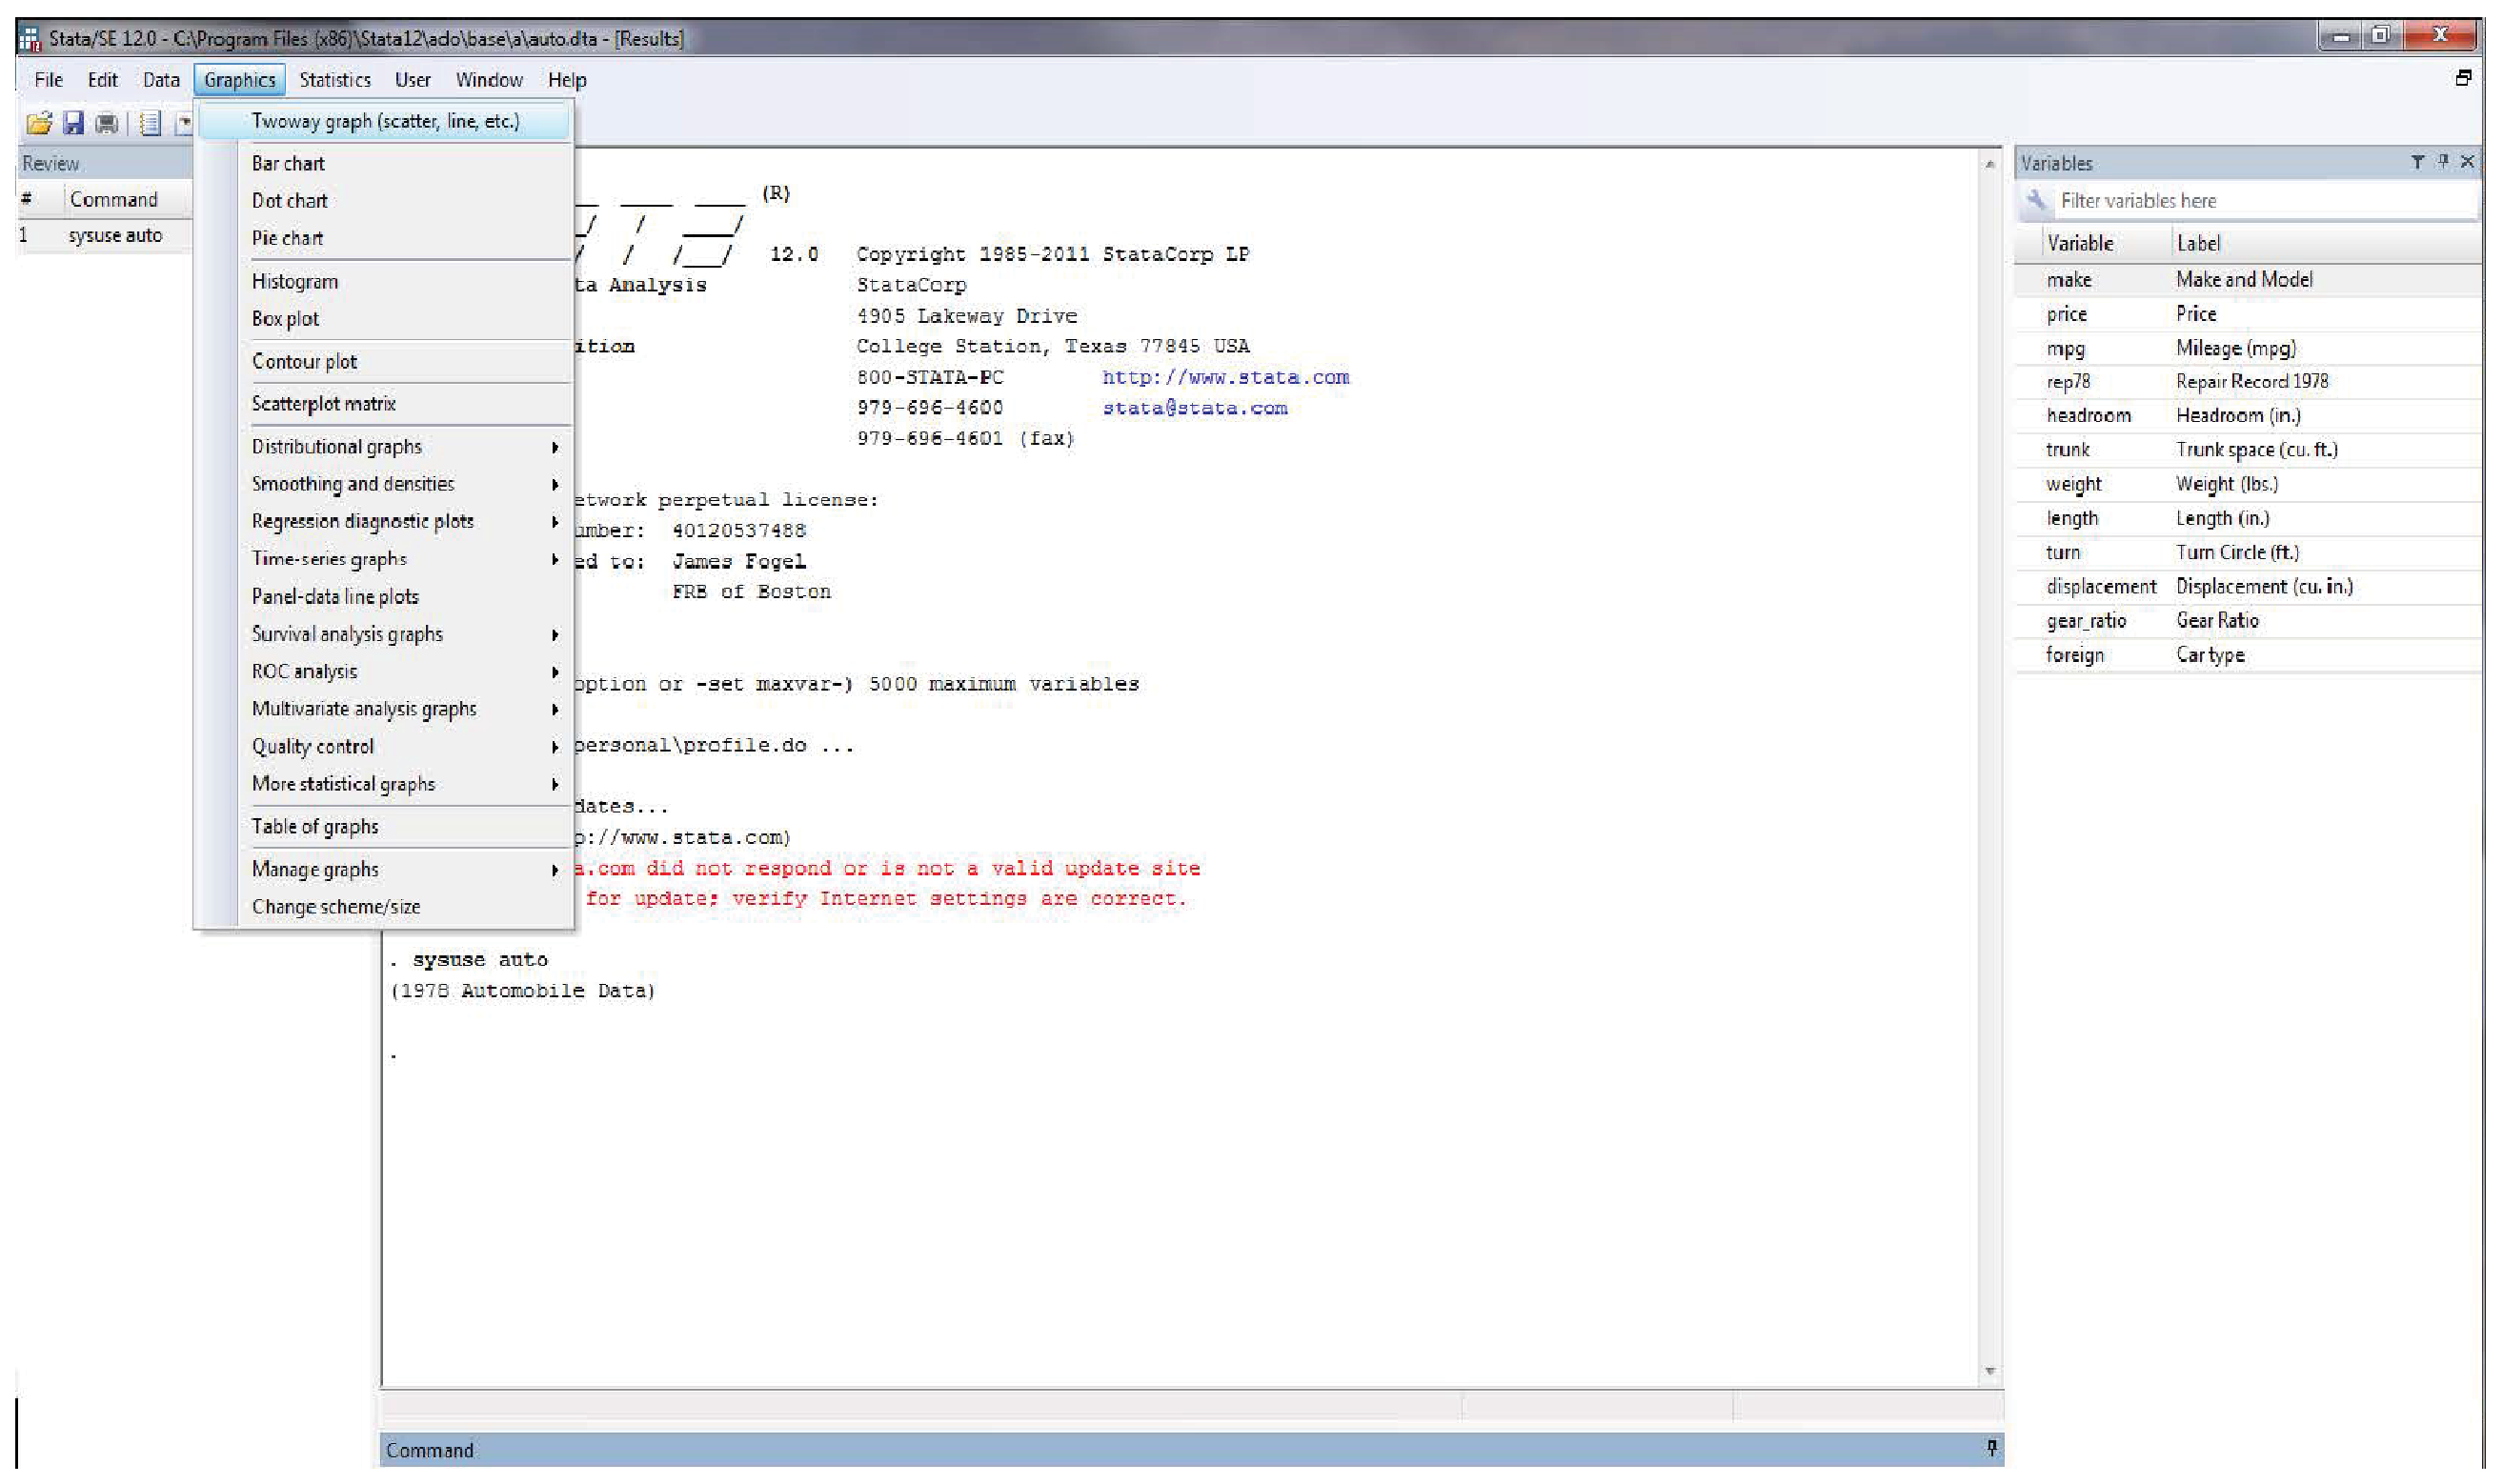
\includegraphics[width=.95\textwidth]{\tex/graphics_dropdown.eps}
\end{frame}

\begin{frame}{Graphics editor}
    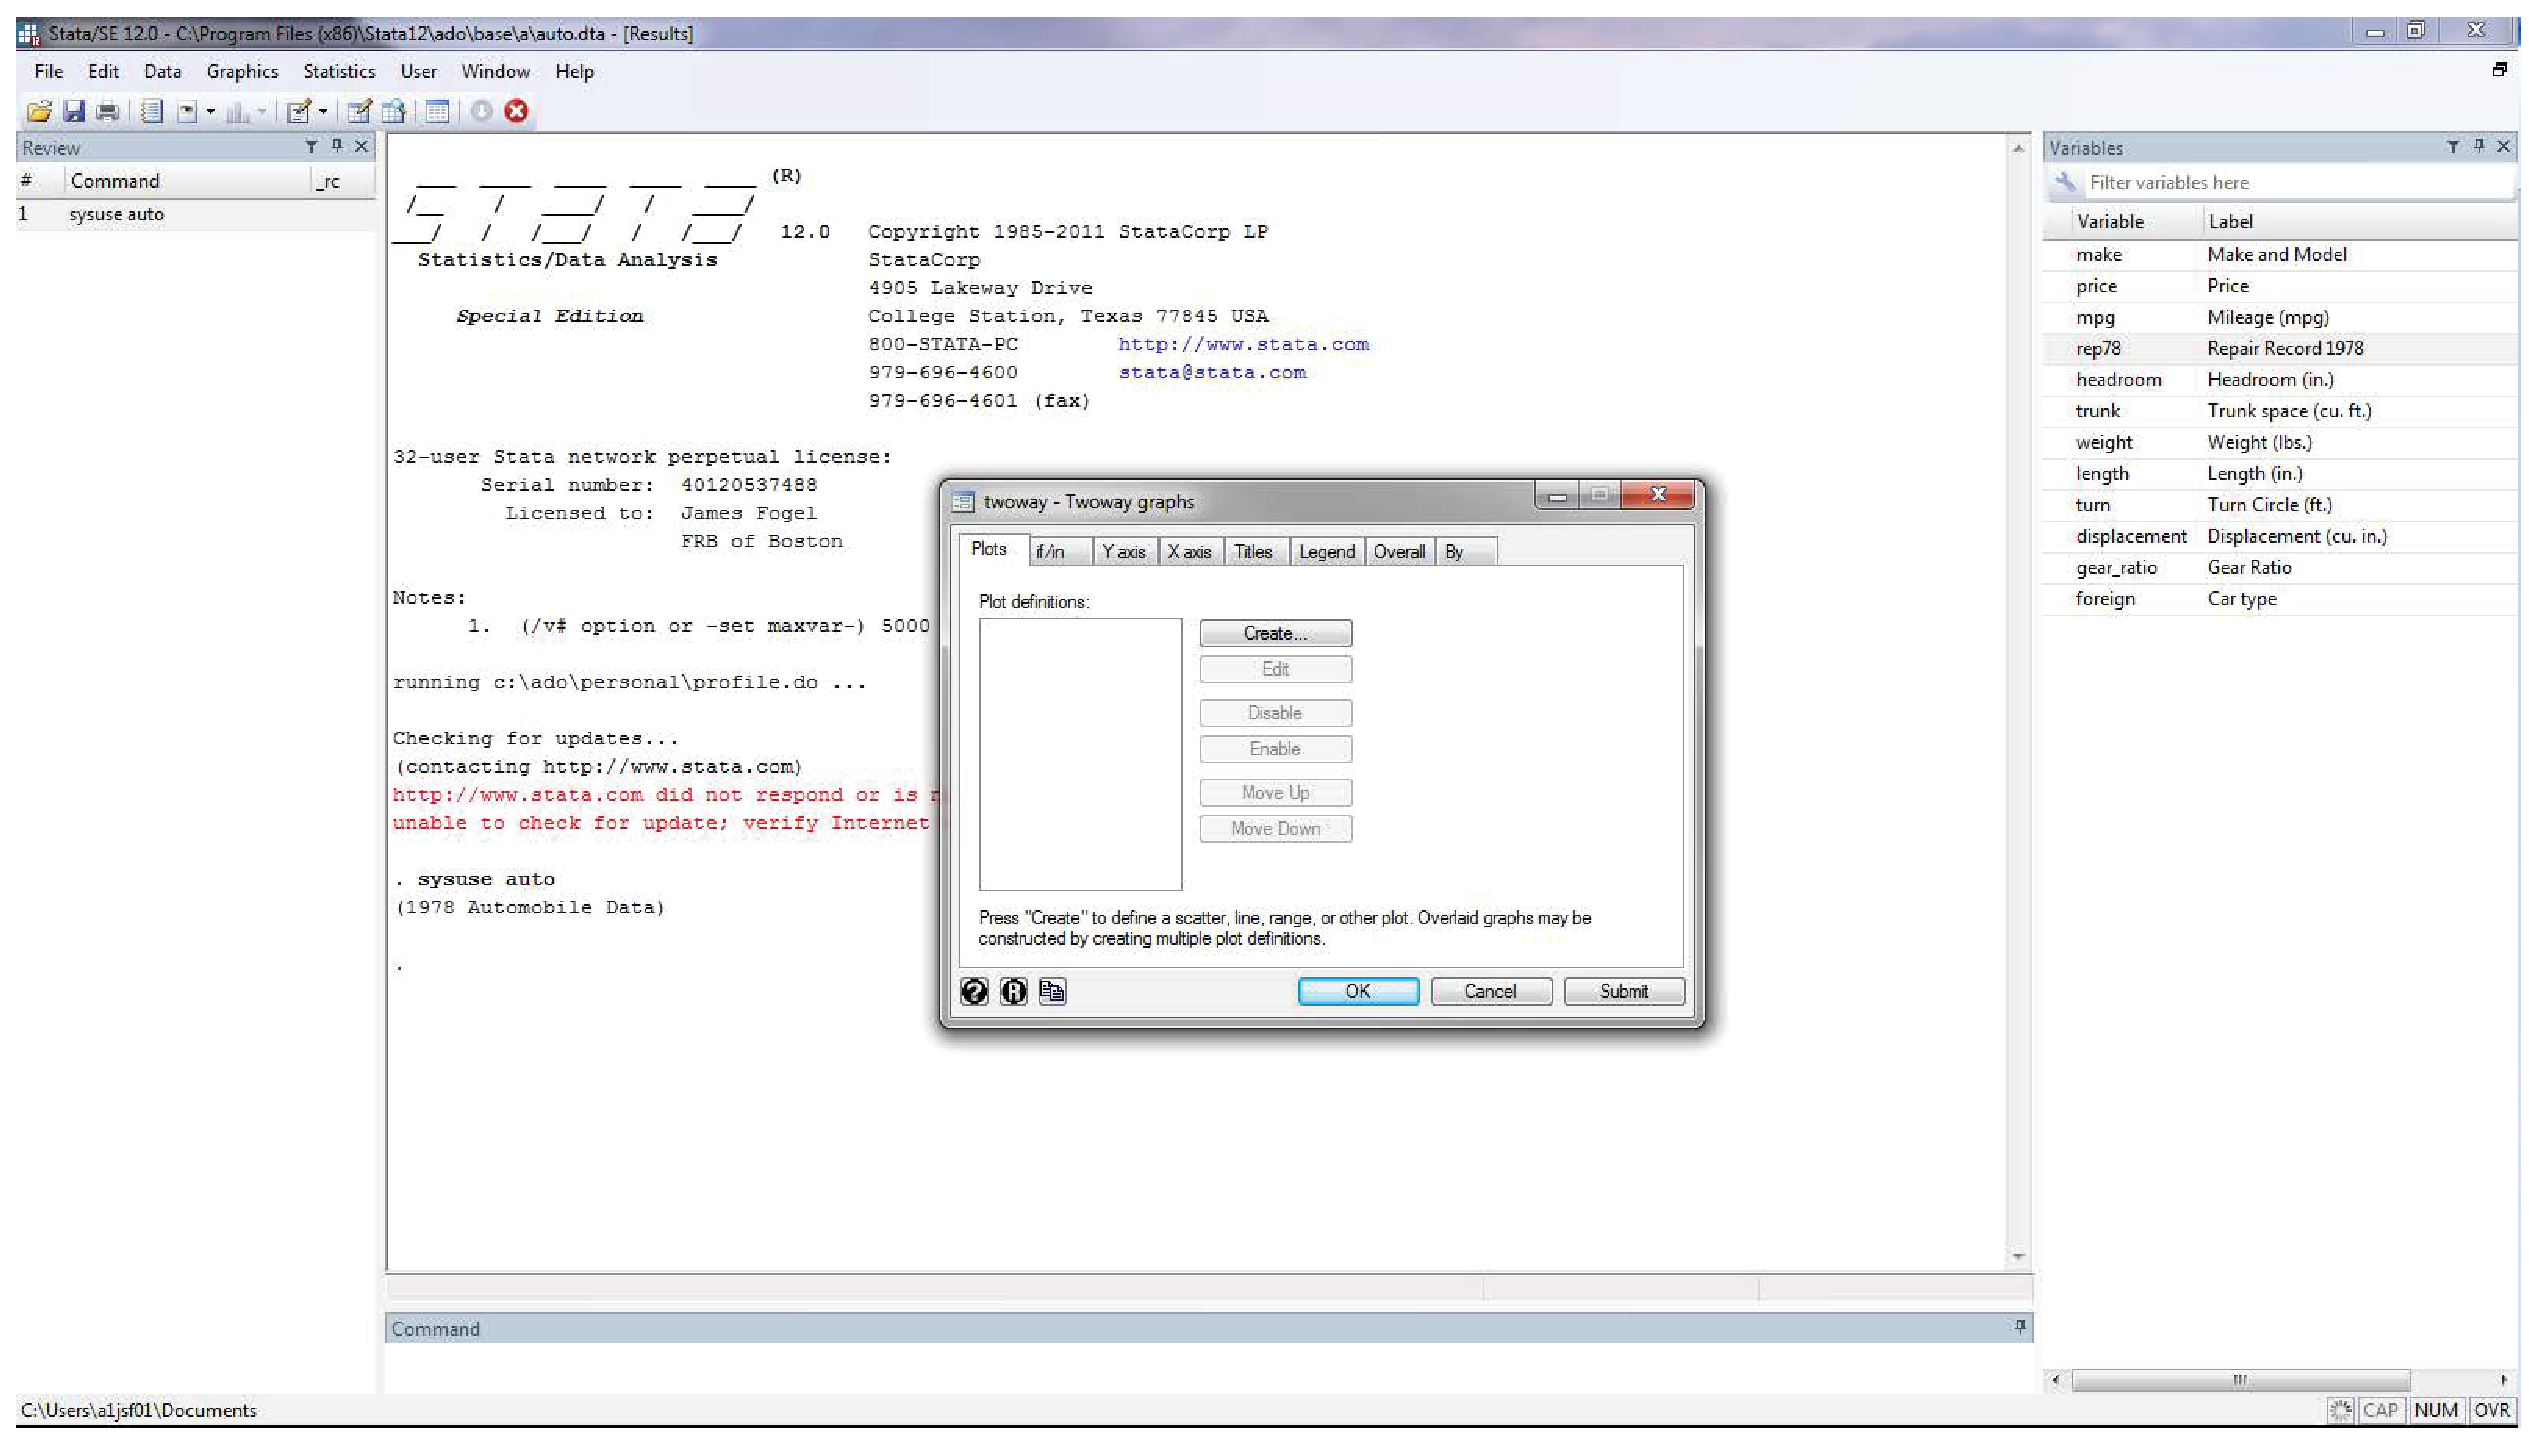
\includegraphics[width=.95\textwidth]{\tex/graphics_editor.eps}
\end{frame}

\begin{frame}{Graphics editor}
    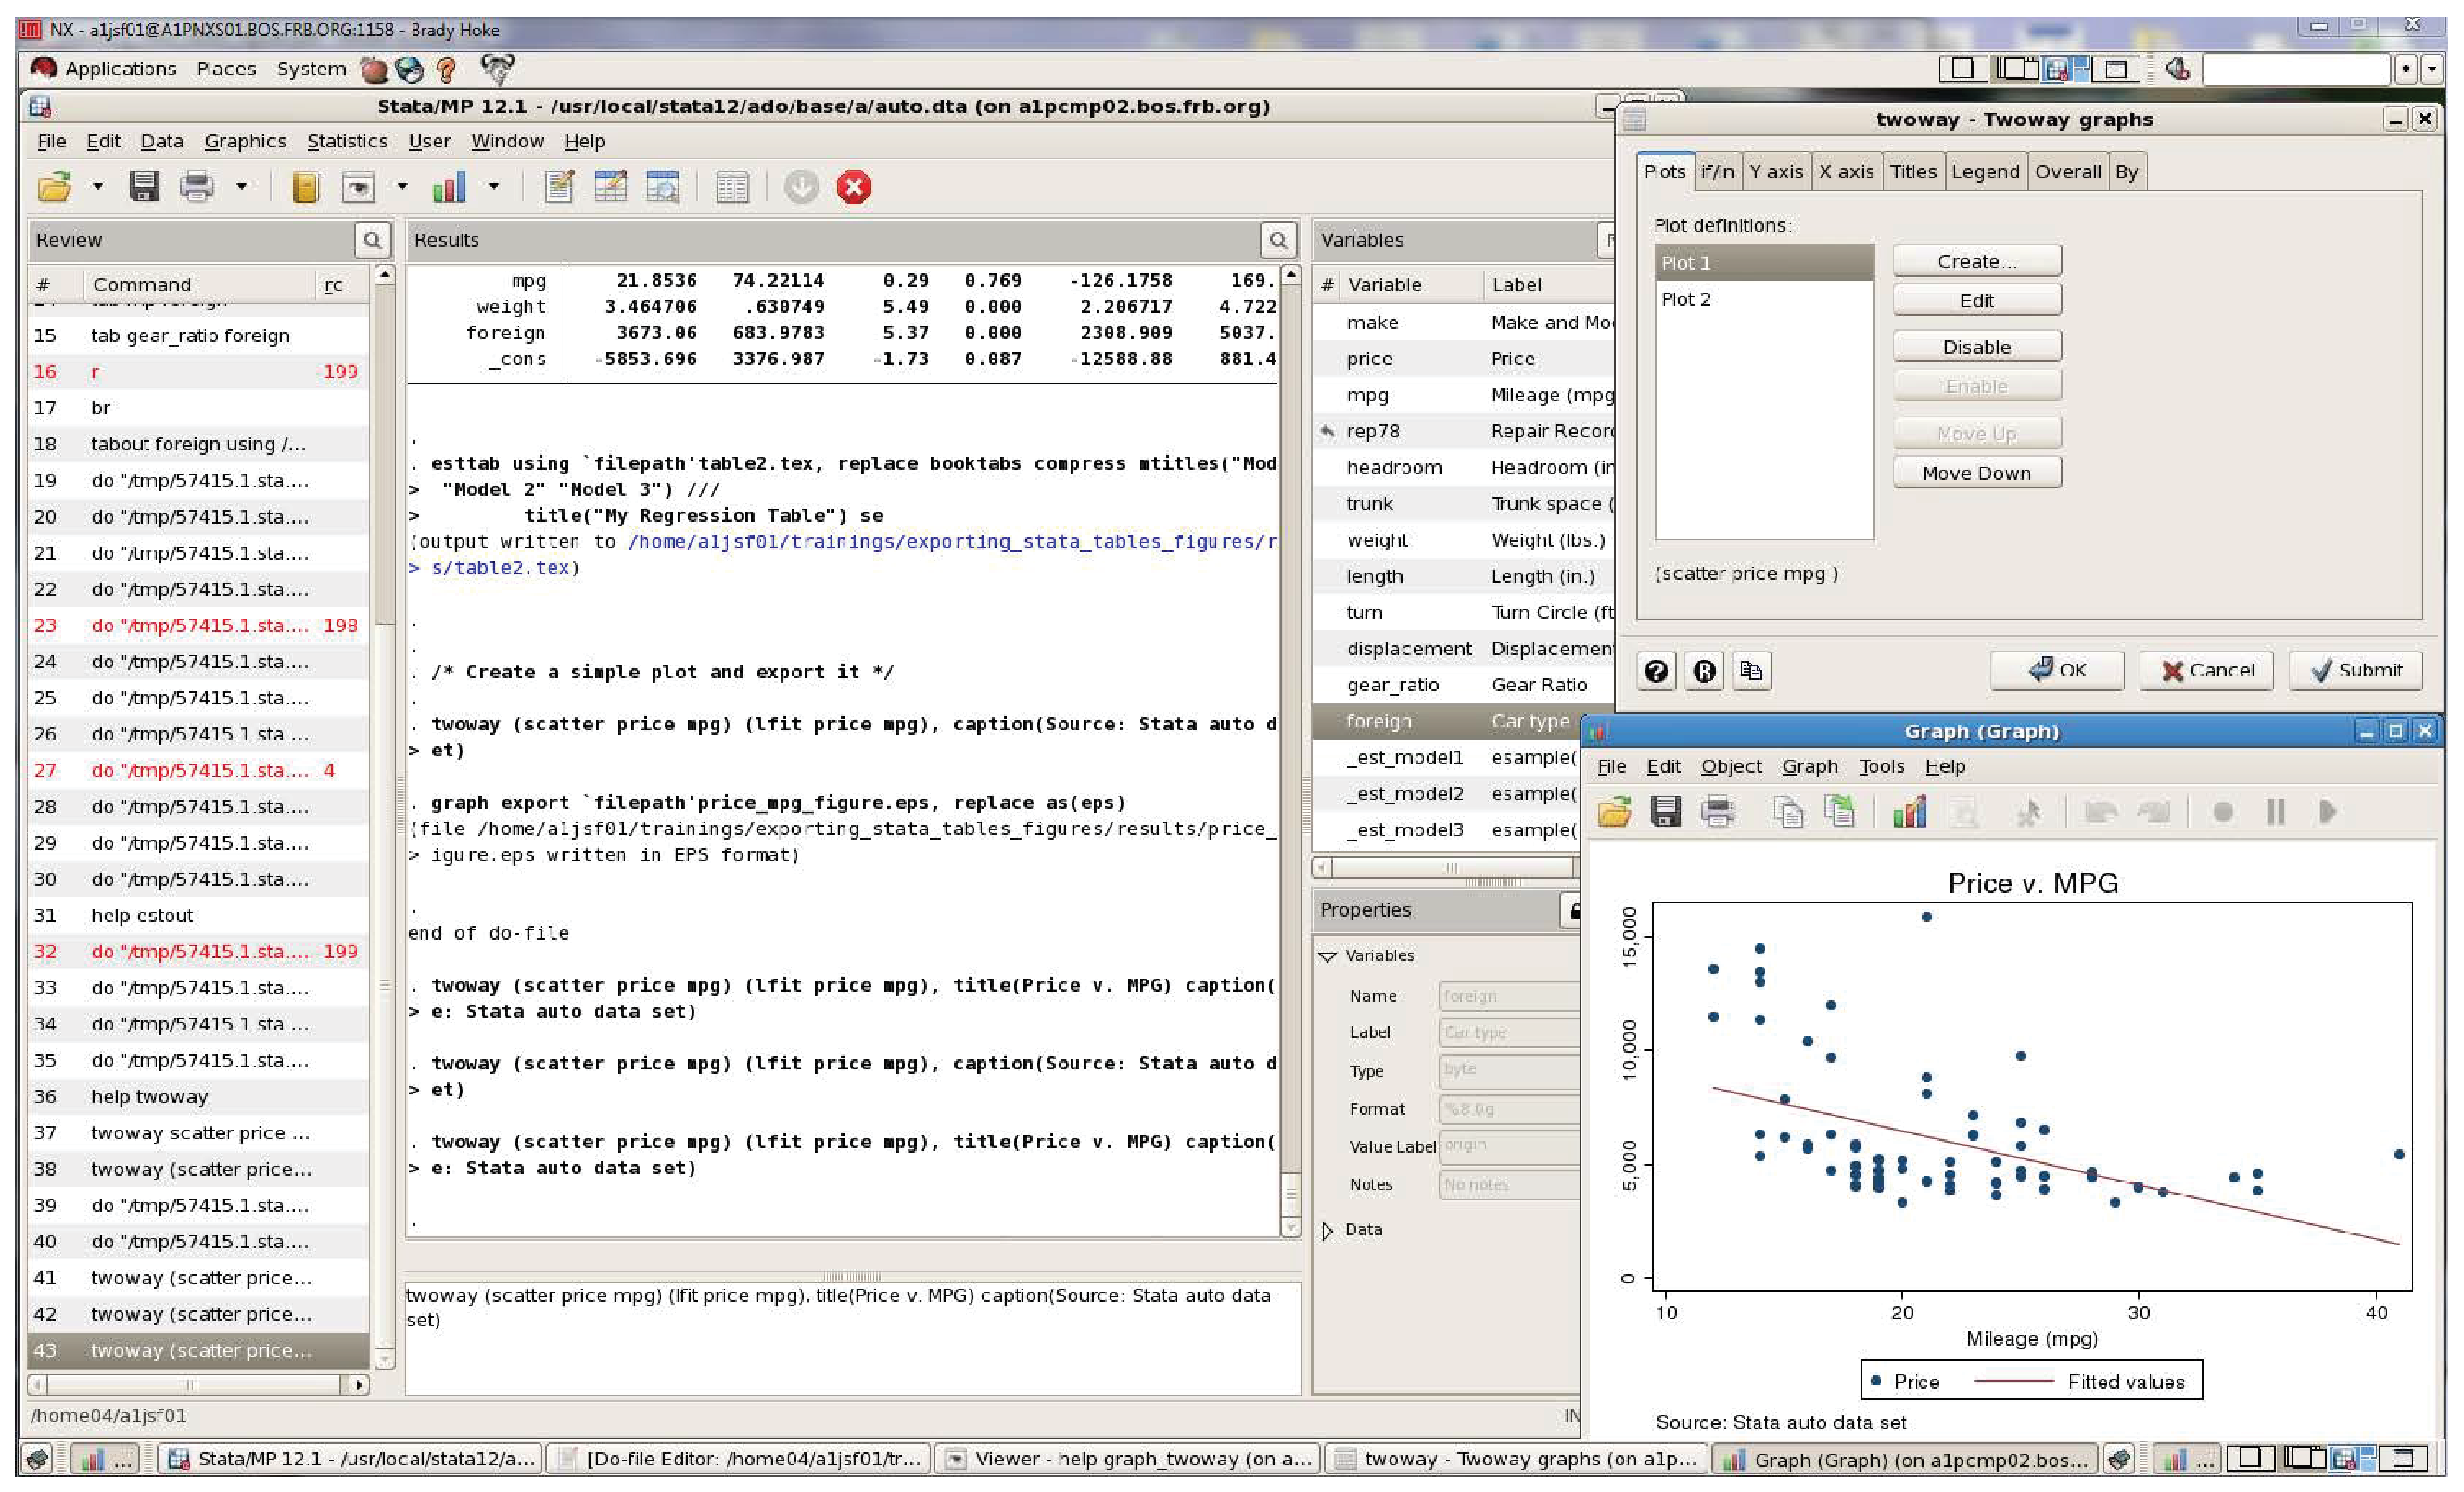
\includegraphics[width=.95\textwidth]{\tex/graphics_results.eps}
\end{frame}


\subsection{Example --- twoway}

\begin{frame}[fragile]{Example --- \lst=twoway=}

 Stata's \lst=twoway= command can be used to combine multiple (compatible) graph types into the same figure; \lst=twoway= takes multiple graph commands as arguments, each in parentheses. In the below example, I use \lst=twoway= to combine a scatter plot and a linear fit:

    \begin{lstlisting}
sysuse auto  //Use Stata's pre-loaded auto data set
twoway (scatter price mpg) (lfit price mpg), title(Price v. MPG) ///
	caption(Source: Stata auto data set)
graph export 'filepath'price_mpg_figure.eps, replace as(eps)
    \end{lstlisting}
	\pause
    \begin{figure}
	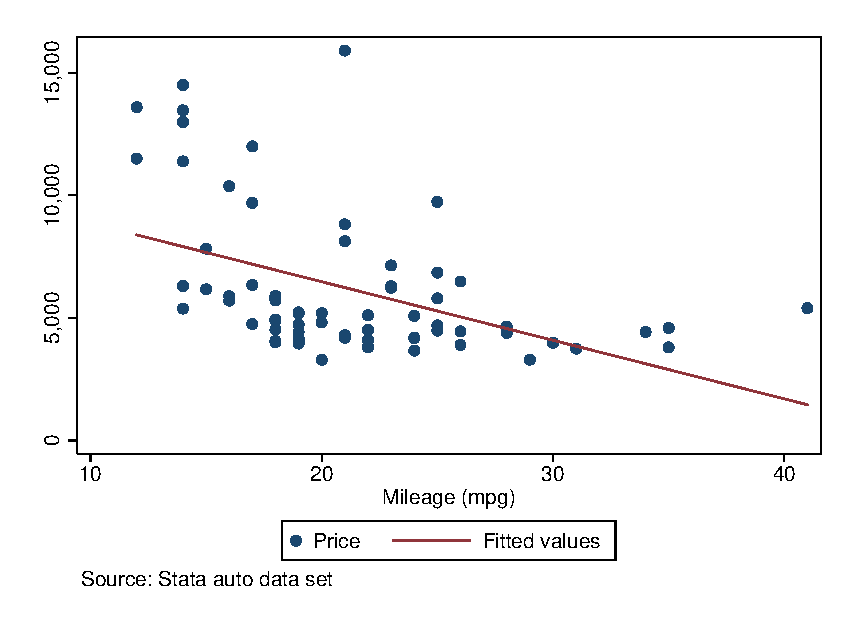
\includegraphics[height=.35\textheight]{\tex/price_mpg_figure.eps}
    \end{figure}
\end{frame}

\subsection{An aside --- Haver}

\begin{frame}{Haver}
    Stata provides a command, \lst=haver use=, that allows you to load data from the Haver Analytics database, provided you know the appropriate mnemonics.

    Unfortunately, \lst=haver use= is compatible with PC Stata only, not Linux Stata. This is an inconvenience, however it is trivially easy to pull and save data using PC Stata and then access it on the Linux Cluster.

    Once we identify a data series, all we need to know is the mnemonic and the file in which it's stored, both of which are listed right below the default chart in Haver.

    \begin{figure}
	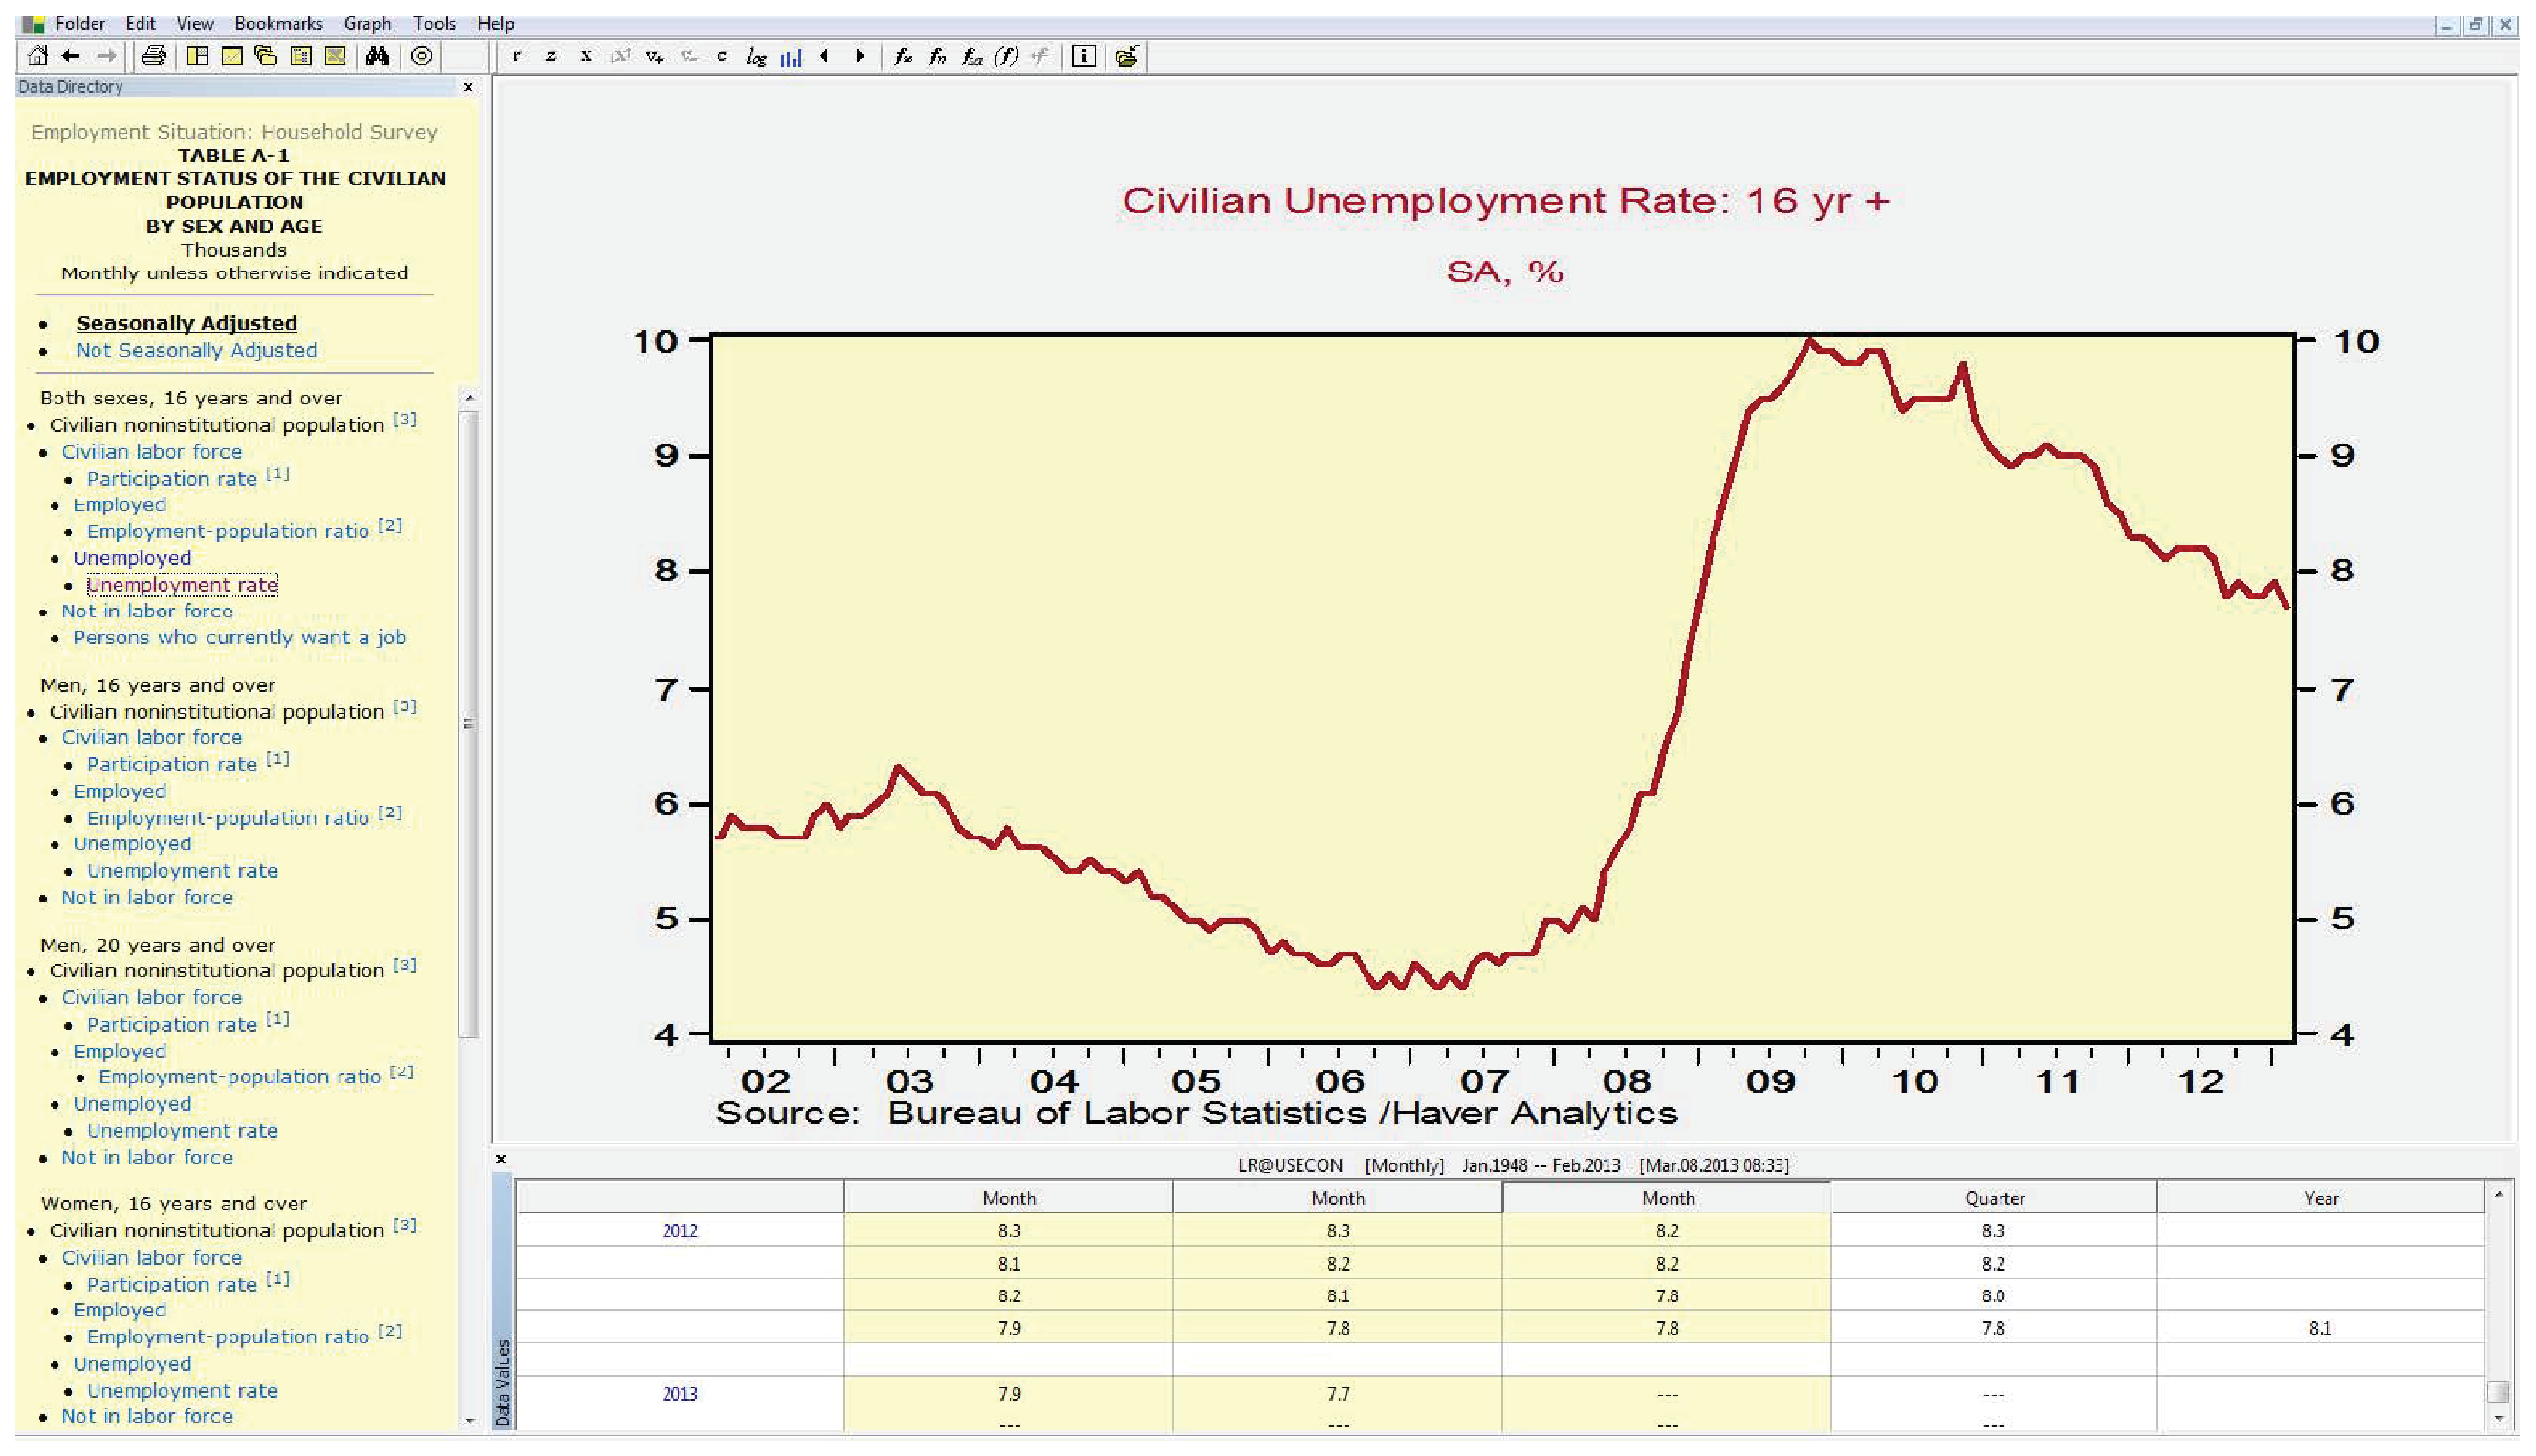
\includegraphics[height=.25\textheight]{\tex/haver_image.eps}
    \end{figure}
\end{frame}

\begin{frame}[fragile]{Haver Example}
    Suppose we want to plot the unemployment rate from January 2000--present, with recession shading. The US unemployment rate is available in Haver under the mnemonic \texttt{LR} in the US Economic Indicators file \texttt{USECON.DAT}, as is the NBER recession indicator (\texttt{RECESSM2}).
    \pause

    \begin{lstlisting}
/* This code will work in PC Stata only */
haver use LR RECESSM2 using "G:\Deptdata\Research\Haver\USECON.DAT", clear

// Formatting date variable
rename time date
format date %tmMon_YY //Format the var so that it will be labeled as a date

// Adjust recession indicator series for consistency with unemployment rate
sum LR
gen recess = (r(max)+1)*RECESSM2

// Plot and export the series
#delimit ;
twoway
  (bar recess date, fintensity(100) lcolor(gs13) fcolor(gs13))
  (tsline LR date)
    \end{lstlisting}
\end{frame}

\begin{frame}{Haver Example}
    \begin{figure}
	   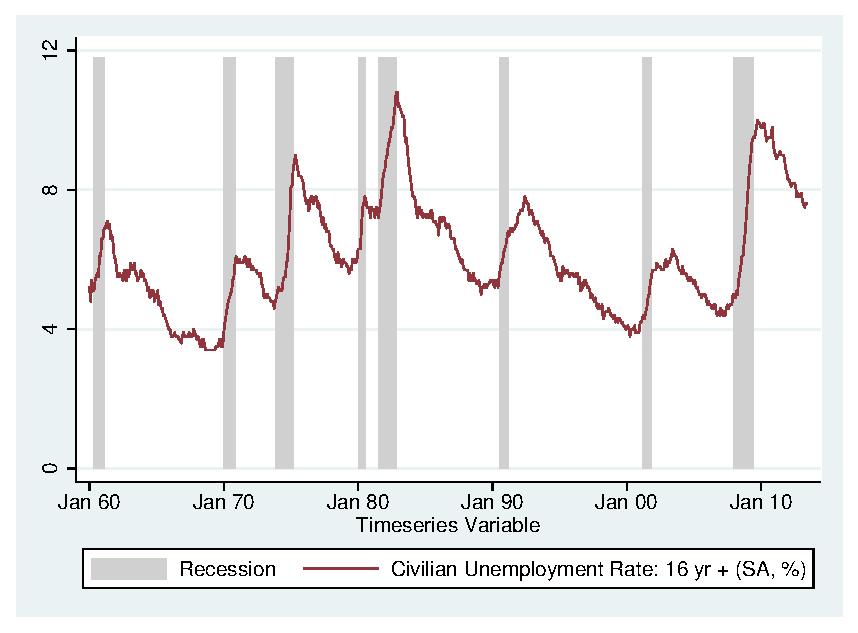
\includegraphics[width=.9\textwidth]{\tex/haver_example.eps}
    \end{figure}
\end{frame}


\subsection{Exporting Graphics}
\begin{frame}[fragile]{\lst=graph export=}
    Stata's \lst=graph export= command allows the user to export the graph currently in memory. Therefore \lst=graph export= usually appears
    immediately after a Stata graph command, such as \lst+twoway tsline varlist+. \lst=graph export= allows you to export graphs as a number
    of different file types, however I usually export figures as .eps files because they are supported by both Linux and Windows Stata and because
    they interact well with \LaTeX{}.
    \begin{lstlisting}
sysuse auto, clear
twoway (scatter price mpg) (lfit price mpg), title(Price v. MPG) ///
    caption(Source: Stata auto data set)
graph export `filepath'price_mpg_figure.eps, replace as(eps)
    \end{lstlisting}

\end{frame}


\subsection{Schemes}

\begin{frame}{Stata provides a number of preset ``schemes'' that define how figures will look. You may also write your own schemes}
    The scheme on the left, s1color\_alt, is a scheme I created myself by adjusting the default colors used by s1color.
    \begin{figure}
	\centering
	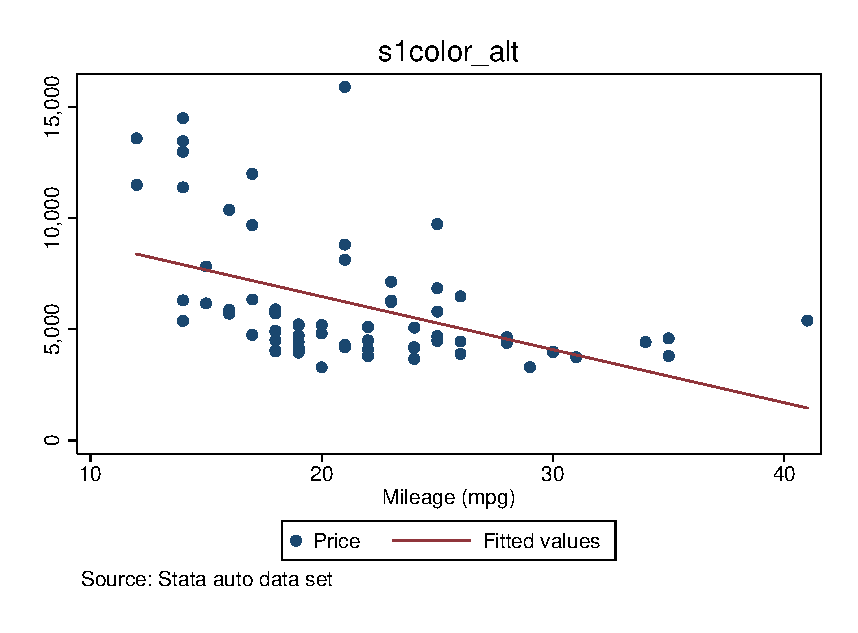
\includegraphics[width=.33\textwidth]{\tex/price_mpg_figure_s1color_alt.eps}
	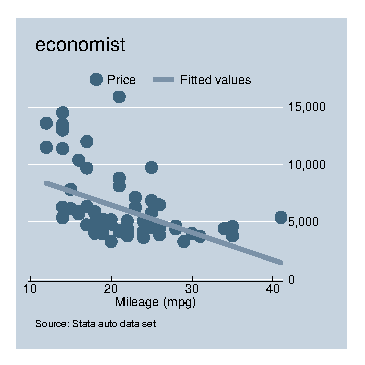
\includegraphics[width=.33\textwidth]{\tex/price_mpg_figure_economist.eps}
	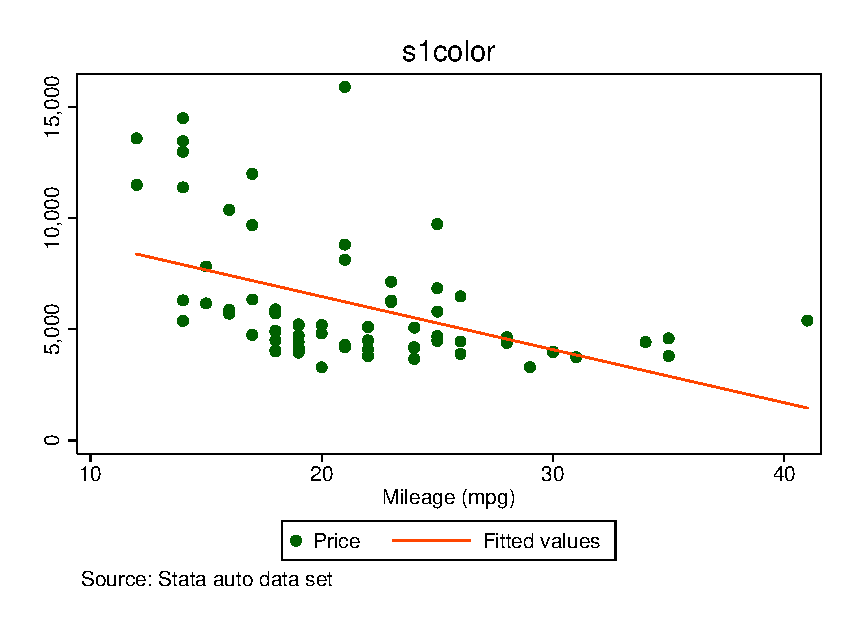
\includegraphics[width=.33\textwidth]{\tex/price_mpg_figure_s1color.eps}
    \end{figure}
\end{frame}


\section{Outputting Results}

\begin{frame}
    Anyone who performs empirical research is familiar with the tedious task of turning estimation output into tables, with appropriate handling of standard errors or t-statistics, p-values, significance stars and presentation of summary statistics. Not only is the task tedious, but any manual manipulation of estimation output opens the door for mistakes, which can create a great deal of extra work for you or cause serious problems if they make it into the final version of a paper or presentation.

    Fortunately, there are a number of user-written packages that greatly improve the process of outputting results. There are a number of useful packages which I will not cover (including a popular one called \lst=outreg2=), however I will focus on two today:
        \begin{enumerate}
    	\item \lst=tabout= --- Outputting tabulations of variables
    	\item \lst=esttab/estout= --- Outputting regression output and other statistical tables
        \end{enumerate}
\end{frame}

\subsection{tabout}


\begin{frame}[fragile]{What is \lst=tabout=?}
     \lst=tabout= allows the user to produce oneway or twoway tables of frequencies and/or percentages, as well as tables of summary statistics. These tables can be exported in a number of different formats, including .csv for use in Excel, but in my opinion the most useful is .tex, which is used by \LaTeX{}. A much more thorough treatment of \lst=tabout= can be found at \url{http://www.ianwatson.com.au/stata/tabout_tutorial.pdf}.
\end{frame}

\begin{frame}[fragile]{A simple tabulation}
    The below command will produce a simple oneway tabulation of the variable \emph{foreign} and save it as a .tex file for use in a \LaTeX{} document: \\
    \vspace{.25cm}
    \begin{lstlisting}
tabout foreign using `filepath'tabout_foreign.tex, replace style(tex)
    \end{lstlisting}
\pause
    \vspace{.25cm}
    \begin{columns}[t]
	\column{.5\textwidth}
	 Code produced by \lst=tabout= \\
	    \begin{lstlisting}
Car type&No. \\
\hline
Domestic&52.0 \\
Foreign&22.0 \\
Total&74.0 \\
	    \end{lstlisting} \pause
	\column{.5\textwidth}
	    Which, when compiled, looks like \\
	    \vspace{.25cm}
	    \begin{tabular}{lr}
		Car type&No. \\
\hline
Domestic&52.0 \\
Foreign&22.0 \\
Total&74.0 \\

	    \end{tabular}
    \end{columns}
\end{frame}


\begin{frame}[fragile]{ Now let's make the table prettier by using the ``booktabs'' option and add a column for the column percentage}

    \vspace{.25cm}
    \begin{lstlisting}
tabout foreign using `filepath'tabout_foreign2.tex, replace style(tex) ///
    cells(freq col) booktabs
    \end{lstlisting}
    \pause
    \begin{columns}[T]
	\column{.5\textwidth}
	    \begin{lstlisting}
Car type&No.&\% \\
\midrule
Domestic&52.0&70.3 \\
Foreign&22.0&29.7 \\
Total&74.0&100.0 \\
	    \end{lstlisting}
	\column{.5\textwidth}
	    \begin{tabular}{lrr}
		 Car type&No.&\% \\
\midrule
Domestic&52.0&70.3 \\
Foreign&22.0&29.7 \\
Total&74.0&100.0 \\

	    \end{tabular}
    \end{columns}
\end{frame}

\begin{frame}[fragile]{We could also do a twoway cross-tab}
    \vspace{.25cm}
    \begin{lstlisting}
tabout foreign over40mpg using `filepath'tabout_foreign_over40mpg.tex, ///
	replace style(tex) cells(freq col)
    \end{lstlisting}
    \pause
    \vspace{.25cm}
    \begin{tabular}{lrrrrrr}
	 & \multicolumn{6}{c}{over40mpg} \\
Car type & \multicolumn{2}{c}{0} & \multicolumn{2}{c}{1} & \multicolumn{2}{c}{Total} \\
&No.&\%&No.&\%&No.&\% \\
\hline
Domestic&52.0&71.2&0.0&0.0&52.0&70.3 \\
Foreign&21.0&28.8&1.0&100.0&22.0&29.7 \\
Total&73.0&100.0&1.0&100.0&74.0&100.0 \\

    \end{tabular}
\end{frame}

\begin{frame}[fragile]{Summary statistics for MPG and weight, broken down by foreign or domestic car}
    \vspace{.25cm}
    \begin{lstlisting}
tabout foreign using `filepath'tabout_sumstats.tex, replace sum ///
	cells(mean mpg	median mpg mean weight median weight) style(tex)}
    \end{lstlisting}
    \pause
    \vspace{.5cm}
    \begin{tabular}{lrrrrrr}
	Car type&Mean&Median&Mean&Median \\
&mpg&mpg&weight&weight \\
\hline
Domestic&19.8&19.0&3,317.1&3,360.0 \\
Foreign&24.8&24.5&2,315.9&2,180.0 \\
Total&21.3&20.0&3,019.5&3,190.0 \\

    \end{tabular}
\end{frame}

\subsection{esttab/estout}


\begin{frame}{What are esttab and estout?}
    \footnotesize{
    The \lst=estout= package is a user-written package which provides tools for producing publication-quality tables in Stata. It contains
    the following programs:
    \begin{itemize}
	\item esttab: Produces publication-style regression tables that display nicely in Stata's results window or, optionally, are exported to formats such as CSV, RTF, HTML, or \LaTeX{}. esttab is a user-friendly wrapper for the estout command. \pause
	\item estout: Generic program to compile a table of coefficients, "significance stars", summary statistics, standard errors, t- or z-statistics, p-values, confidence intervals, or other statistics for one or more models previously fitted and stored. The table is displayed in the results window or written to a text file. \pause
	\item eststo: Utility to store estimation results for later tabulation. eststo is an alternative to official Stata's estimates store. Main advantages of eststo over estimates store are that the user does not have to provide a name for the stored estimation set and that eststo may be used as a prefix command. \pause
	\item estadd: Program to add extra results to the returns of an estimation command. This is useful to make the the results available for tabulation. \pause
	\item estpost: Program to prepare results from commands such as summarize, tabulate, or correlate for tabulation by esttab or estout. \pause
    \end{itemize}
    }
    \footnotesize For further details see \url{http://repec.org/bocode/e/estout/index.html} or \\ \url{http://repec.org/bocode/e/estout/esttab.html}
\end{frame}

\begin{frame}{esttab}
    For the most part you will want to use \lst=esttab= rather than \lst=estout= because it produces nicely-formatted tables suitable
	for export as \LaTeX{}, CSV, RTF, or HTML formats. All of \lst=estout='s options are also available in \lst=esttab=, however the
	reverse is not true. Additionally, \lst=esttab= produces all of the code for opening the table and tabular environment that we had
	to provide ourselves when using tabout.
\end{frame}

\begin{frame}[fragile]{Let's produce a simple regression table using the auto data set.}

    \vspace{1cm}
    \begin{columns}[T]
	\column{.5\linewidth}
	    \footnotesize{
	    \begin{lstlisting}
sysuse auto, clear
eststo clear
eststo: reg price mpg weight
eststo: reg price mpg foreign
eststo: reg price mpg weight foreign
esttab using `filepath'table1.tex, ///
    replace booktabs compress	   ///
    addnote("Your footnote here")
	    \end{lstlisting}
	    }
\pause
	\column{.5\linewidth}
	    \tiny{
		{
\def\sym#1{\ifmmode^{#1}\else\(^{#1}\)\fi}
\begin{tabular}{l*{3}{c}}
\toprule
          &\multicolumn{1}{c}{(1)}&\multicolumn{1}{c}{(2)}&\multicolumn{1}{c}{(3)}\\
          &\multicolumn{1}{c}{price}&\multicolumn{1}{c}{price}&\multicolumn{1}{c}{price}\\
\midrule
mpg       &   -49.51         &   -294.2\sym{***}&    21.85         \\
          &  (-0.57)         &  (-5.28)         &   (0.29)         \\
\addlinespace
weight    &    1.747\sym{**} &                  &    3.465\sym{***}\\
          &   (2.72)         &                  &   (5.49)         \\
\addlinespace
foreign   &                  &   1767.3\sym{*}  &   3673.1\sym{***}\\
          &                  &   (2.52)         &   (5.37)         \\
\addlinespace
\_cons    &   1946.1         &  11905.4\sym{***}&  -5853.7         \\
          &   (0.54)         &  (10.28)         &  (-1.73)         \\
\midrule
\(N\)     &       74         &       74         &       74         \\
\bottomrule
\multicolumn{4}{l}{\footnotesize \textit{t} statistics in parentheses}\\
\multicolumn{4}{l}{\footnotesize Your footnote here}\\
\multicolumn{4}{l}{\footnotesize \sym{*} \(p<0.05\), \sym{**} \(p<0.01\), \sym{***} \(p<0.001\)}\\
\end{tabular}
}

	    }
    \end{columns}
\end{frame}

\begin{frame}[fragile]{Alternatively, we could explicitly name each set of regression estimates and \lst=esttab= any combination of the stored estimation sets.}

    \vspace{1cm}
    \begin{columns}[T]
	\column{.5\linewidth}
	    \footnotesize{
	    \begin{lstlisting}
sysuse auto, clear
eststo clear
eststo e1: reg price mpg
eststo e2: reg price mpg weight
eststo e3: reg price mpg foreign
eststo e4: reg price mpg weight foreign
esttab e2 e3 e4			   ///
    using `filepath'table1.tex,	   ///
    replace booktabs compress	   ///
    addnote("Your footnote here")
	    \end{lstlisting}
	    }
	\column{.5\linewidth}
	    \tiny{
		{
\def\sym#1{\ifmmode^{#1}\else\(^{#1}\)\fi}
\begin{tabular}{l*{3}{c}}
\toprule
          &\multicolumn{1}{c}{(1)}&\multicolumn{1}{c}{(2)}&\multicolumn{1}{c}{(3)}\\
          &\multicolumn{1}{c}{price}&\multicolumn{1}{c}{price}&\multicolumn{1}{c}{price}\\
\midrule
mpg       &   -49.51         &   -294.2\sym{***}&    21.85         \\
          &  (-0.57)         &  (-5.28)         &   (0.29)         \\
\addlinespace
weight    &    1.747\sym{**} &                  &    3.465\sym{***}\\
          &   (2.72)         &                  &   (5.49)         \\
\addlinespace
foreign   &                  &   1767.3\sym{*}  &   3673.1\sym{***}\\
          &                  &   (2.52)         &   (5.37)         \\
\addlinespace
\_cons    &   1946.1         &  11905.4\sym{***}&  -5853.7         \\
          &   (0.54)         &  (10.28)         &  (-1.73)         \\
\midrule
\(N\)     &       74         &       74         &       74         \\
\bottomrule
\multicolumn{4}{l}{\footnotesize \textit{t} statistics in parentheses}\\
\multicolumn{4}{l}{\footnotesize Your footnote here}\\
\multicolumn{4}{l}{\footnotesize \sym{*} \(p<0.05\), \sym{**} \(p<0.01\), \sym{***} \(p<0.001\)}\\
\end{tabular}
}

	    }
    \end{columns}
\end{frame}

\begin{frame}[fragile]{\lst=esttab= flexibility}
    \lst=esttab= allows the user a great deal of flexibility in formatting tables. For example, we can add model titles, a caption, and replace the t-statistics with standard errors.
    {\footnotesize
    \begin{lstlisting}
esttab using `filepath'table2.tex, replace booktabs compress ///
    mtitles("Model 1" "Model 2" "Model 3") ///
    title("My Regression Table") se
    \end{lstlisting}
    }
    {\tiny
    \begin{table}[htbp]\centering
\def\sym#1{\ifmmode^{#1}\else\(^{#1}\)\fi}
\caption{My Regression Table}
\begin{tabular}{l*{3}{c}}
\toprule
          &\multicolumn{1}{c}{(1)}&\multicolumn{1}{c}{(2)}&\multicolumn{1}{c}{(3)}\\
          &\multicolumn{1}{c}{Model 1}&\multicolumn{1}{c}{Model 2}&\multicolumn{1}{c}{Model 3}\\
\midrule
mpg       &   -49.51         &   -294.2\sym{***}&    21.85         \\
          &  (86.16)         &  (55.69)         &  (74.22)         \\
\addlinespace
weight    &    1.747\sym{**} &                  &    3.465\sym{***}\\
          &  (0.641)         &                  &  (0.631)         \\
\addlinespace
foreign   &                  &   1767.3\sym{*}  &   3673.1\sym{***}\\
          &                  &  (700.2)         &  (684.0)         \\
\addlinespace
\_cons    &   1946.1         &  11905.4\sym{***}&  -5853.7         \\
          & (3597.0)         & (1158.6)         & (3377.0)         \\
\midrule
\(N\)     &       74         &       74         &       74         \\
\bottomrule
\multicolumn{4}{l}{\footnotesize Standard errors in parentheses}\\
\multicolumn{4}{l}{\footnotesize \sym{*} \(p<0.05\), \sym{**} \(p<0.01\), \sym{***} \(p<0.001\)}\\
\end{tabular}
\end{table}

    }
\end{frame}

\begin{frame}{A few key points about outputting results}
    \begin{itemize}
	 \item \textbf{You should \emph{NEVER} be copying and pasting Stata output from the results window or a log file!} \pause
	 \item The only way to learn \lst=tabout= and \lst=esttab= is to start using them, dig through the documentation, Google your questions, or ask other RAs for help. You will pick them up quickly. \pause
	 \item Once you have spent some time using \lst=tabout= and \lst=esttab= you will have built up your own library of templates, which you will be able to copy, paste, and make minor edits to for future use!
    \end{itemize}
\end{frame}

\section{Programs \& Ado-files}

\subsection{Introduction}

\begin{frame}{Programs \& Ado-files}
    First, some Stata nomenclature:
    \begin{enumerate}
        \item Stata formally defines a program as a set of Stata commands that includes a \lst=program= statement.
        \item An \textbf{ado-file} is simply a file that stores a program (see, for example, \lst{viewsource estout.ado}
    \end{enumerate}

    You can easily write a Stata program, stored in an ado-file, that handles all the features of official Stata commands such as the \lst=if= and \lst=in= options. You can even write a help file that documents its operation, for your benefit and for those with whom you share the code.

    \textbf{But you probably shouldn’t!} In most cases, existing Stata commands —-- official or user-written --— will perform the tasks you need. Use Stata's search features such as \lst=findit= and the Stata user community (Statalist) to ensure that the program you envision has not already been written.
\end{frame}

\subsection{Creating an Ado-file}

\begin{frame}[fragile]
    A Stata program adds a command to Stata’s language. The name of the program is the command name, and the program must be stored in a file of that same name with extension .ado, and placed on the adopath — i.e., the list of directories that Stata will search to locate programs. A program begins with the \lst=program define program_name= statement, which usually includes the option \lst=, rclass=. The program name should not be the same as any Stata command, nor the same as any accessible user-written command!

    The \lst=syntax= command will almost always be used to define the command’s format. For instance, a command that accesses one or more variables in the current data set will have a \lst=syntax varlist= statement. The \lst=syntax= statement does allow you to specify \lst=[if]= and \lst=[in]= arguments, which allow commands to limit the observations used. The \lst=syntax= statement may also include a \lst=using= qualifier, allowing your command to read or write files. Really, any feature you find in an official Stata command can be implemented with an appropriate \lst=syntax= statement.
\end{frame}

\begin{frame}[fragile]
    A sample program from \lst=help return=:
    \begin{lstlisting}
program mysum, rclass
    syntax varname
    tempvar new
    quietly {
        count if !missing(`varlist')
        return scalar N = r(N)
        gen double `new' = sum(`varlist')
        return scalar sum = `new'[_N]
        return scalar mean = return(sum)/return(N)
    }
end
    \end{lstlisting}
    This program can be executed as \lst=mysum varname=. It prints nothing but places three scalars in the return list. The values \lst=r(N)=, \lst=r(sum)=, and \lst=r(mean)= can now be referred to directly.
    \begin{lstlisting}
mysum mpg
display r(N) "  " r(sum) "  " r(mean)
>74  1576  21.297297
    \end{lstlisting}
\end{frame}


\section{Mata}

\subsection{Introduction}

\begin{frame}{Mata --- Stata's very own matrix programming language!}
    Stata contains a full-blown matrix language, \emph{Mata}, with many of the capabilities of MATLAB and R. Why should you care?
    \begin{enumerate}
        \item Mata is automatically compiled into bytecode and hence runs many times faster than the standard Stata language.
        \item Mata circumvents the limitations of Stata's traditional matrix commands
        \item Mata contains a large library of mathematical and matrix functions, including optimization routines, equation solvers, decompositions, and probability density functions.
    \end{enumerate}
    I am not going to dwell on Mata syntax in this training --- it is largely similar to C and its handling of matrices is broadly similar to that of other matrix languages like MATLAB or R (see \lst=help mata=).
\end{frame}

\subsection{Example --- OLS}

\begin{frame}[fragile]
    \begin{lstlisting}
sysuse auto , clear

// Entering Mata
mata
// Defining matrices
x = st_data(., ("mpg"))
y = st_data(., ("price"))
cons = J(rows(x), 1, 1)
X = (x, cons)

// Some linear algebra
beta_hat = ( invsym(X’*X))*(X’*y)
e_hat = y - X * beta_hat
s2 = (1 / (rows(X) - cols(X))) * (e_hat ’ * e_hat )
V_ols = s2 * invsym (X ’*X)
se_ols = sqrt(diagonal(V_ols))

// Returning results
st_matrix ("beta_hat", beta_hat)
st_matrix ("se_ola", se_ols)
// Leaving Mata
end
    \end{lstlisting}
\end{frame}

\begin{frame}
    But you should never program OLS (or something equally simple) in Mata. \textbf{Why?} \pause

    Stata has already programmed it for you in its \lst=regress= command! You do not want to write redundant commands or code because it is a waste of time, may contain errors, is unlikely to be as efficient as the commands Stata or other users have written, and because when you share your code with someone else, they will have a much easier time understanding your code if you stick to standard Stata commands.

    Writing your own programs and Mata code can be very useful, but only when you know that you will be performing the same operation over and over and you are confident that no one else has written code that will accomplish the same task.
\end{frame}

\section{Miscellaneous}

\subsection{Time Series, Panels, and Categorical/Factor Variables}

\begin{frame}[fragile]{Declaring data to be time series or panel data}
    A number of commands are built specifically for time series data (everything in the \lst=TS= manual) or panel data (te \lst=xt= manual).
    \begin{itemize}
        \item \lst=tsset= --- declare data set to be time series data (see \lst=help tsset=)
        \item \lst=xtset= --- declare data set to be panel data (see \lst=help xtset=)
    \end{itemize}
\end{frame}


\begin{frame}[fragile]{Special operators for time series and factor variables}
    \begin{itemize}
        \item Stata provides lag (\lst=L.=, lead (\lst=F.=), difference (\lst=D.=) and other special operators for time series variables. See \lst=help tsvarlist= for more details.
        \item Stata also provides special operators for factor variables and interactions. See \lst=help fvvarlist= for more details.
        \item The \lst=xi= command creates a full set of dummy variables out of categorical variables. See \lst=help xi= for more details.
    \end{itemize}
\end{frame}

\subsection{Automating Data Downloads (Linux Stata)}

\begin{frame}[fragile]{Automating Data Downloads (Linux Stata)}
    Downloading files from a website is easy to automate if the files are stored in a systematic way. This is a good practice for several reasons — it makes the task more efficient, well documented, and easily replicable. Generally, the actual downloading takes place outside of the Stata application, but Stata can coordinate the downloads using local variables and invoking shell commands (see previous section) within a loop. Perhaps the simplest Linux command to quickly download a file is the \lst=wget= command, which downloads the path it is provided (for example, \lst+wget "http://www.example.com/file.dat"+). The \lst=wget= command also has many other options to enhance its functionality.

    For example, to download ten years of annual CSV data one might write:
    \begin{lstlisting}
forvalues year = 2000/2010 {
    !wget "http://www.example.com/`year'data.csv"
}
    \end{lstlisting}
\end{frame}

\subsection{Debugging}
\begin{frame}[fragile]{Debugging}
   \begin{itemize}
      \item \lst=pause= --- \lst=pause= will pause execution of your code and return control of Stata. You may continue execution from that point by typing \lst=end= or break execution with \lst=BREAK=.
      \item \lst=trace= --- \lst=trace= displays each line from each ado file it runs. It allows you to see exactly what is going on within each command you use. Unfortunately, \lst=trace= produces a large amount of output that can be difficult to sift through.
      \item \lst=findbug= --- \lst=findbug= is a user-written command that is a nice replacement for \lst=trace=. \lst=findbug= keeps a trace of of the execution of your code and, if an error occurs, displays the line that triggered the error along with several preceding and succeeding lines.
    \end{itemize}	
\end{frame}

\subsection{Capture, confirm, and assert}

\begin{frame}[fragile]{\lst=capture=}
    \lst=capture= executes a command, suppressing all its output (including error messages, if any) and issues a return code of zero.  The actual return  code generated by command is stored in the built-in scalar \_rc.

    Capture is useful if you know that a command may cause an error message but you would like to disregard the message and continue execution. For example suppose you want to close any open log file, but you aren't sure that a log file is open: \lst capture log close=.
\end{frame}

\begin{frame}[fragile]{\lst=assert= and \lst=confirm=}
    \lst=assert= tests whether or not a condition is true and generates an error message if it is false. It is a very useful tool for ensuring that your code is running as you expect it should. For example, \lst=assert _merge==3= after a merge will check that all observations merged successfully and will generate an error if not.

    \lst=confirm= may be used to verify that files or variables exist and/or are of the expected type.
\end{frame}

\subsection{Managing Licenses on the Cluster}
\begin{frame}{Managing Licenses on the Linux Cluster}
    We only have 25 licenses for Linux Stata so if you use more than you need you may prevent someone else from using Stata. We have about 45 economists and RAs so it is very important to not waste licenses.
\end{frame}

\begin{frame}[fragile]{Use the Stata Launch utility to run multiple sessions on one license}
    \includegraphics[width=.9\textwidth]{\tex/stata_launch.eps}
\end{frame}

\begin{frame}[fragile]{You can check your license usage with the \lst=!qstat= command}
    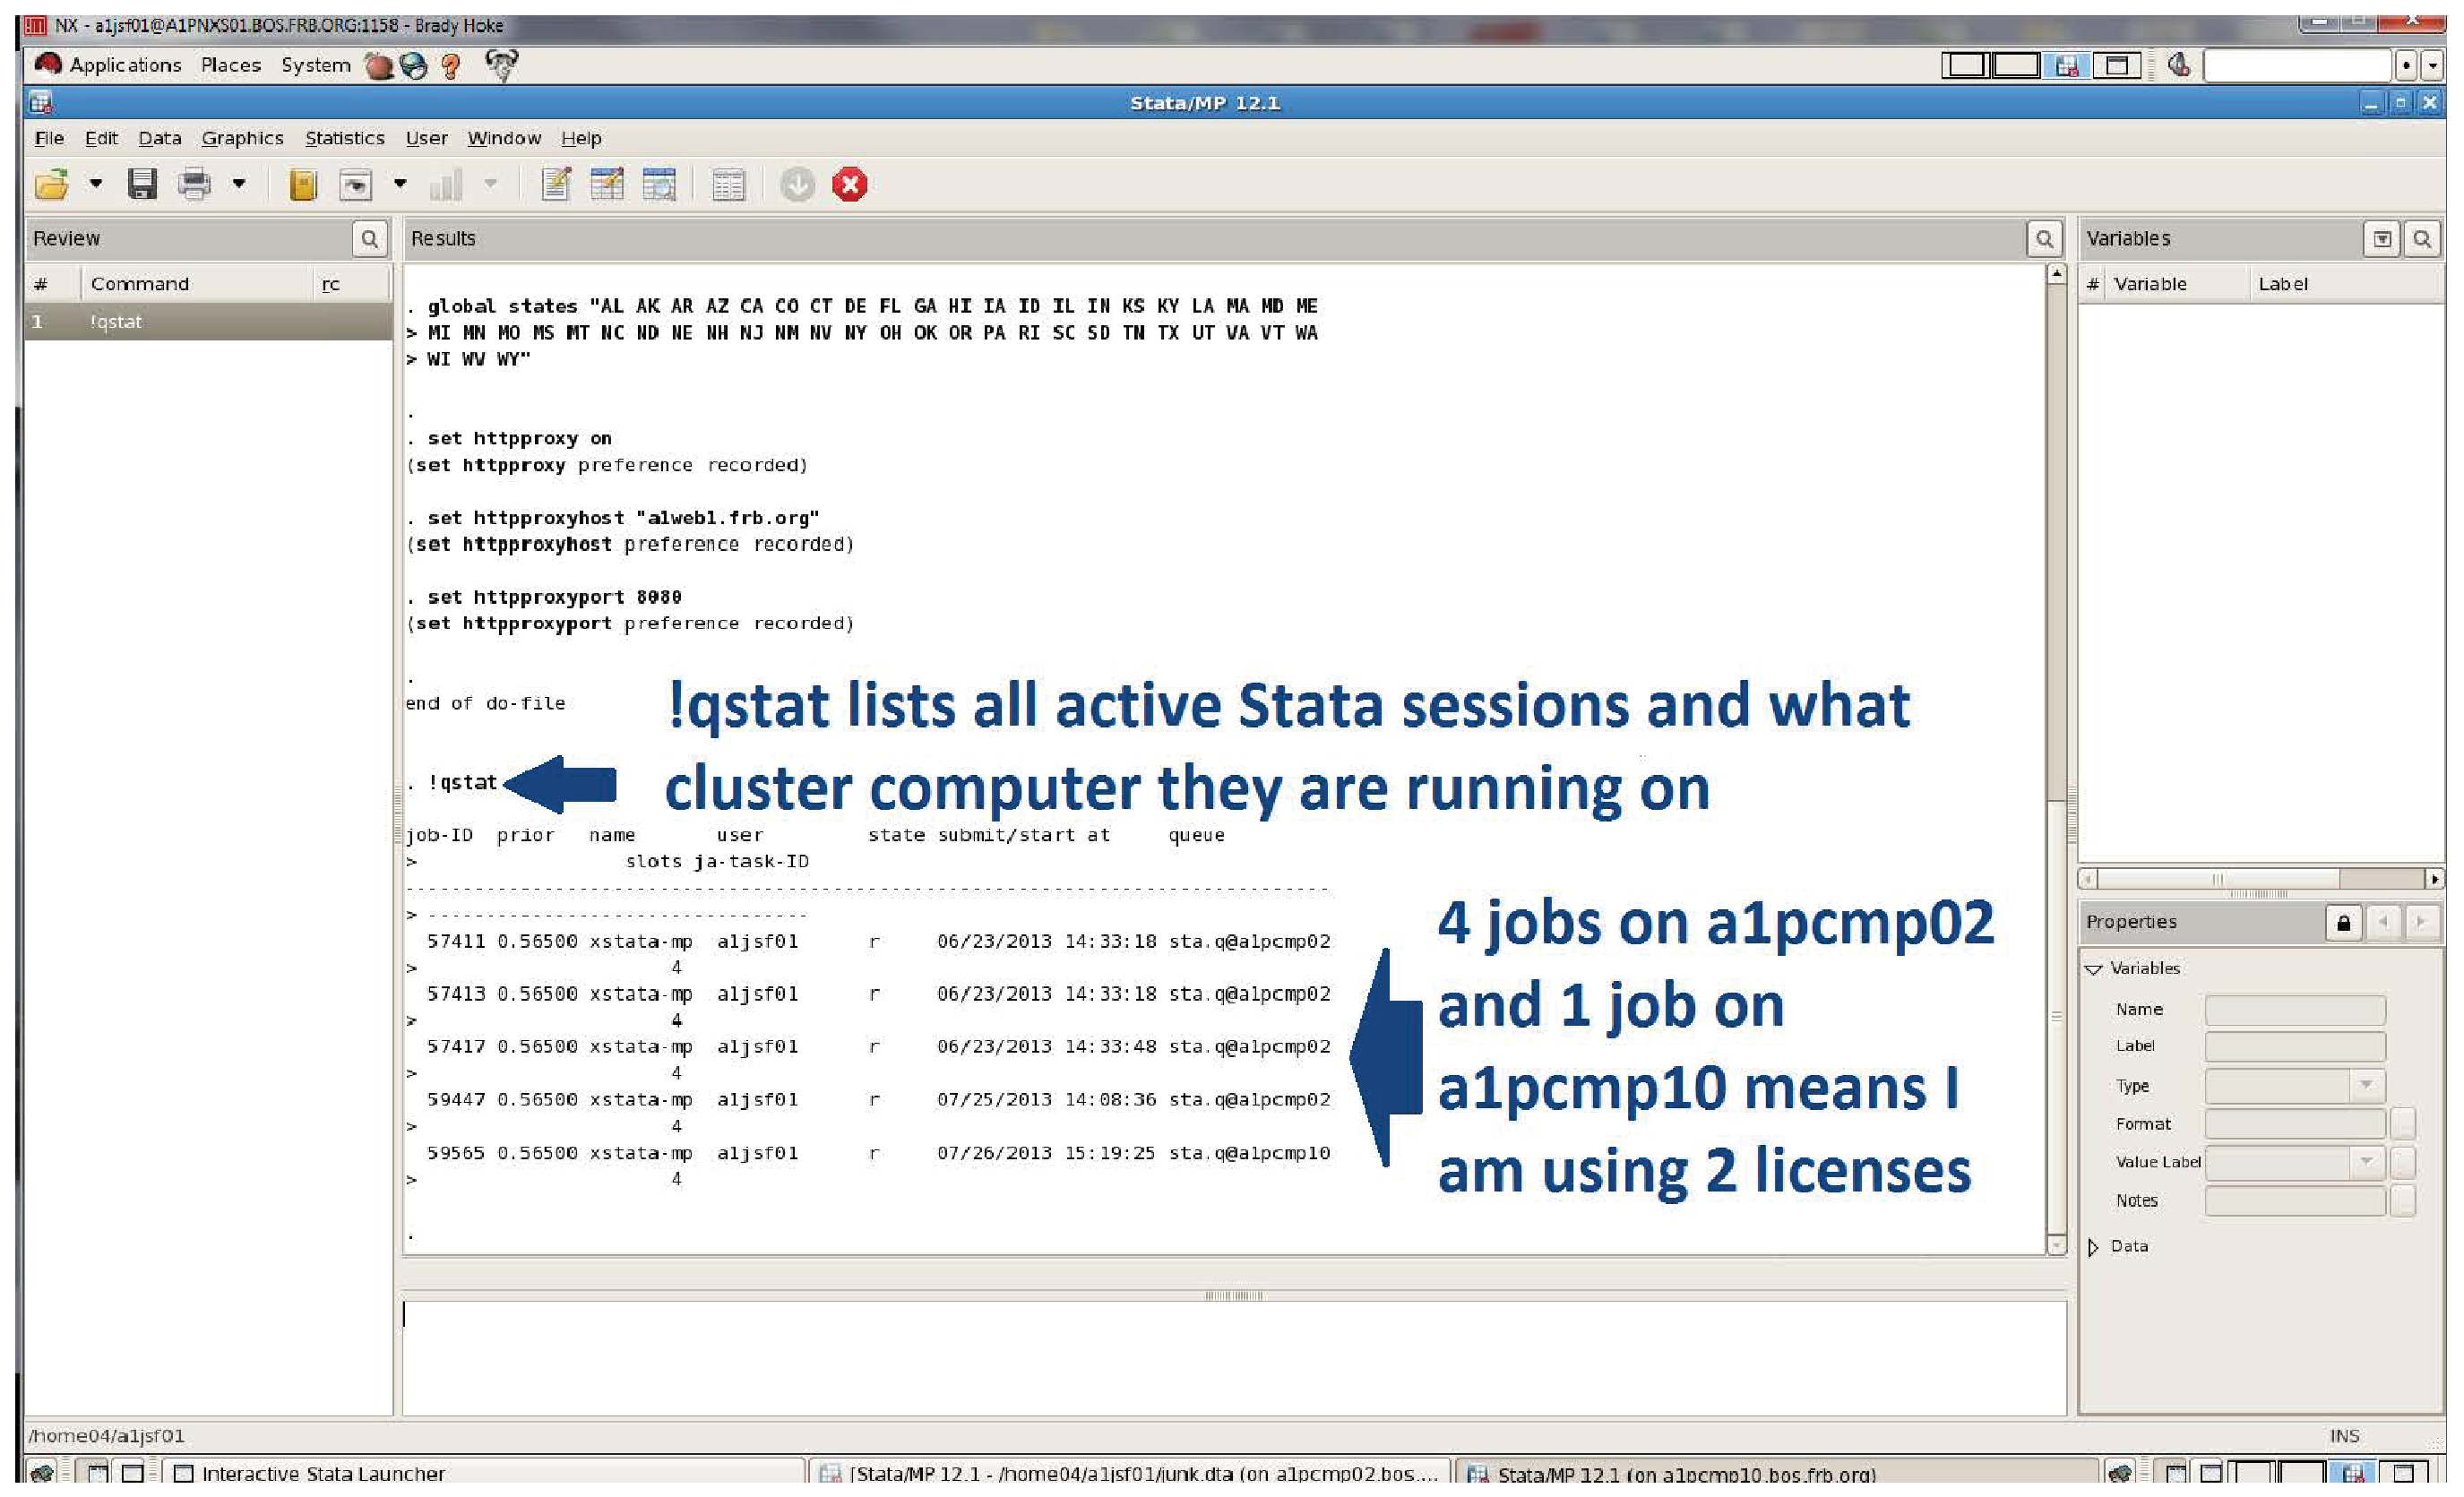
\includegraphics[width=.9\textwidth]{\tex/qstat.eps}
\end{frame}

\begin{frame}[fragile]{Batch Stata}
    Instead of running Stata interactively, you may submit individual jobs in batch mode. In batch mode Stata executes your do-file entirely behind the scenes and creates a log file to keep track of execution. Batch mode uses a license only while Stata is executing and immediately relinquishes that license once execution completes. Batch mode is ideal for running do-files that take a long time but don't need to be actively monitored, such as do-files that automate large data set creation tasks or perform complex and time-consuming estimation routines.

    To run Stata in batch mode open the terminal window and enter at the command line:
    \begin{lstlisting}
qbatch stata filepath/yourdofile.do
    \end{lstlisting}
    Speak with Jones for further details.
\end{frame}

\section{Stata Resources}

\begin{frame}{Stata Resources}
    Have questions? Use the following resources:
    \begin{enumerate}
        \item Stata help files
        \item Google
        \item Stata manuals (located by CLS on T-8)
        \item Other RAs
        \item Statalist (be sure to read the Statalist FAQ’s before posting!).
    \end{enumerate}
\end{frame}


\end{document}

